\chapter{Introduction}

\section{Enzyme catalysts are required to sustain cellular life}
Life on earth is dependent on the chemical synthesis of molecules, which constitute the building blocks of cellular organisms. Early proto-organisms had to adopt a way in which they could ensure a constant nutrient supply, without which life would be unlikely to persist on geological time scales. The selective pressure for auxotropy witnessed the emergence of essential chemical reactions that convert naturally available nutrients into various molecules to support specific functions. This included the provision of a wide variety of molecules suitable for the many complex anabolic and catabolic reactions essential for the support of organismic growth and division such as sugars, lipids, nucleotides and amino acids. The ability to perform chemical synthesis is achieved through pathways of sequential reactions collectively known as metabolism, and subsequently rendered organisms non-reliant on specific geochemical conditions enabling them to colonise a diversity array of ecological niches.

\subsection{The evolutionary emergence of biological catalysts}
Metabolism can be viewed as a network of inter-connected chemical reactions, whose topological features are largely conserved in all studied organisms. Two important inferences can be drawn from the highly conserved nature of metabolic reactions: (i) metabolic networks likely reached a state of efficiency very early on in evolutionary time scales that could barely be improved further by natural selection, and (ii) all present forms of metabolism likely descend from the same original network \cite{Jeong:2000aa}. These conclusions give rise to the hypothesis, originally proposed by Aleksandr Oparin in his 1938 book 'The Origin of Life' \cite{oparin1965origin}, that a common metabolic network topology dates back to non-enzymatic chemistry in the presence of simple inorganic ions as found in the highly reducing geochemical environment that made up the Archaen sediment. Indeed, metabolic intermediates of two pathways in central carbon metabolism - glycolysis and the pentose phosphate pathway (PPP) - were shown to undergo non-enzymatic interconversion in chemical compositions replicating the pre-biotoic Archaen ocean \cite{Keller:2014aa}. Additionally, ions that were abundant in the Archaean sediment, such as $Fe^{2+}$ and $PO^{3-}$, can catalyse reactions which are reminiscent of the modern PPP, suggesting that modern metabolic reactions did not necessarily result from the evolutionary selection of complex enzyme catalysts, but rather that such reactions were able to proceed under prevailing chemical conditions in the Archaean sea \cite{Ralser:2014aa}. 
%
%
\\\\
%
%
Small molecules such as metal ions can efficiently catalyse many chemical reactions. Several constraints on biological systems, however, render their utility insufficient for supporting complex cellular life \textit{per se}. Many metal ion catalysts found at high concentrations in the Archaean ocean, do not accumulate to sufficient concentrations in modern biological conditions, such that they can function as efficient catalysts. For example, ferrous iron is readily water soluble in the absence of oxygen, and anoxic conditions in the earth's early surface environment resulted in the Archaean milieu preserving a high iron content, whereas its oxidised form was readily depleted upon the great oxygenation event \cite{Konhauser:2011aa}. This likely imposed a strong selection pressure for species to evolve their metabolism, becoming less dependent on the presence of increasingly rare and/or insoluble molecules, eventually leading to the emergence of macromolecular catalysts. 
%
%
\\\\
%
%
The RNA world hypothesis provides a conceptual framework whereby the emergence of genetic selection can be explained by RNA molecules acting as self-replicators, thereby unifying heritability and the propensity for stochastic evolution \cite{Orgel:2004aa}. Indeed, RNA molecules have been used in directed evolution experiments and, in a milestone paper, Lincoln and Joyce (2009) \cite{Lincoln:2009aa} presented an experimentally designed \textit{in vitro} self-replicating RNA enzyme. Nevertheless, the ability for RNA enzymes to catalyse reactions, other than phosphoester cleavage or ligation, is limited. The design of an RNA enzyme by Fusz \textit{et al.} (2005) \cite{Fusz:2005aa} that could act as an intermolecular catalyst of the aldol reaction was found to be $Zn^{2+}$-dependent. Peptides can also bind to metal ions, and simple metal-binding RNA or peptide structures could provide the starting point for positive selection by supporting multiple reactions, and would have prevented the loss of low concentrations of metal ions through diffusion and/or precipitation \cite{Ralser:2014aa}. A likely consequence of non-enzymatic metabolism was that early enzyme and RNA catalysts were able to evolve in the background of non-specific metal ion-catalysed reactions. To avoid the production of superoxide from hydrogen peroxide by ferrous iron, modern cells evolved a complex iron transport mechanism to prevent accumulation of ferrous iron in the cytoplasm \cite{aisen1980iron}. Subsequently, peptide and RNA secondary structures would have increased the affinity for some substrates, facilitating access to the retained metal catalyst, giving rise to early enzymes. 
%
%
\\\\
%
%
A dynamic chemical system operating at typical biological rates, with all intermediates at concentrations in the nanomolar to millimolar range, can be constructed only by use of efficient catalysts. The emergence of enzyme catalysts enabled metabolism to cope with the high demand for biomass, necessary to sustain the requirements of cellular organisms (\textbf{Fig. \ref{fig:biol_catalysts}}). Enzymes can achieve unrivalled substrate specificity due to their complex protein folds and can distinguish between very similar compounds, which prevents the progression of undesirable side-reactions \cite{Ralser:2014aa}. In addition to greater fidelity, the phenomenon of enzyme substrate specificity frequently results in the binding of metabolites, which closely resemble the natural substrate, to the active site of the enzyme, resulting in a steric preclusion of the natural substrate from the catalytic site. This phenomenon manifests as competitive inhibition, and provides an example of how the kinetic properties of enzyme catalysts can be reversibly regulated. Compared to small-molecule catalysts, whose catalytic activity is not readily regulated, the complex three-dimensional structure of enzymes houses pockets which allow metabolites and other small molecules to bind and regulate enzyme activity. The implications of enzyme regulation for metabolism are discussed in the following section. 
%
%
%%% FIGURE
%
\begin{figure}[!ht]
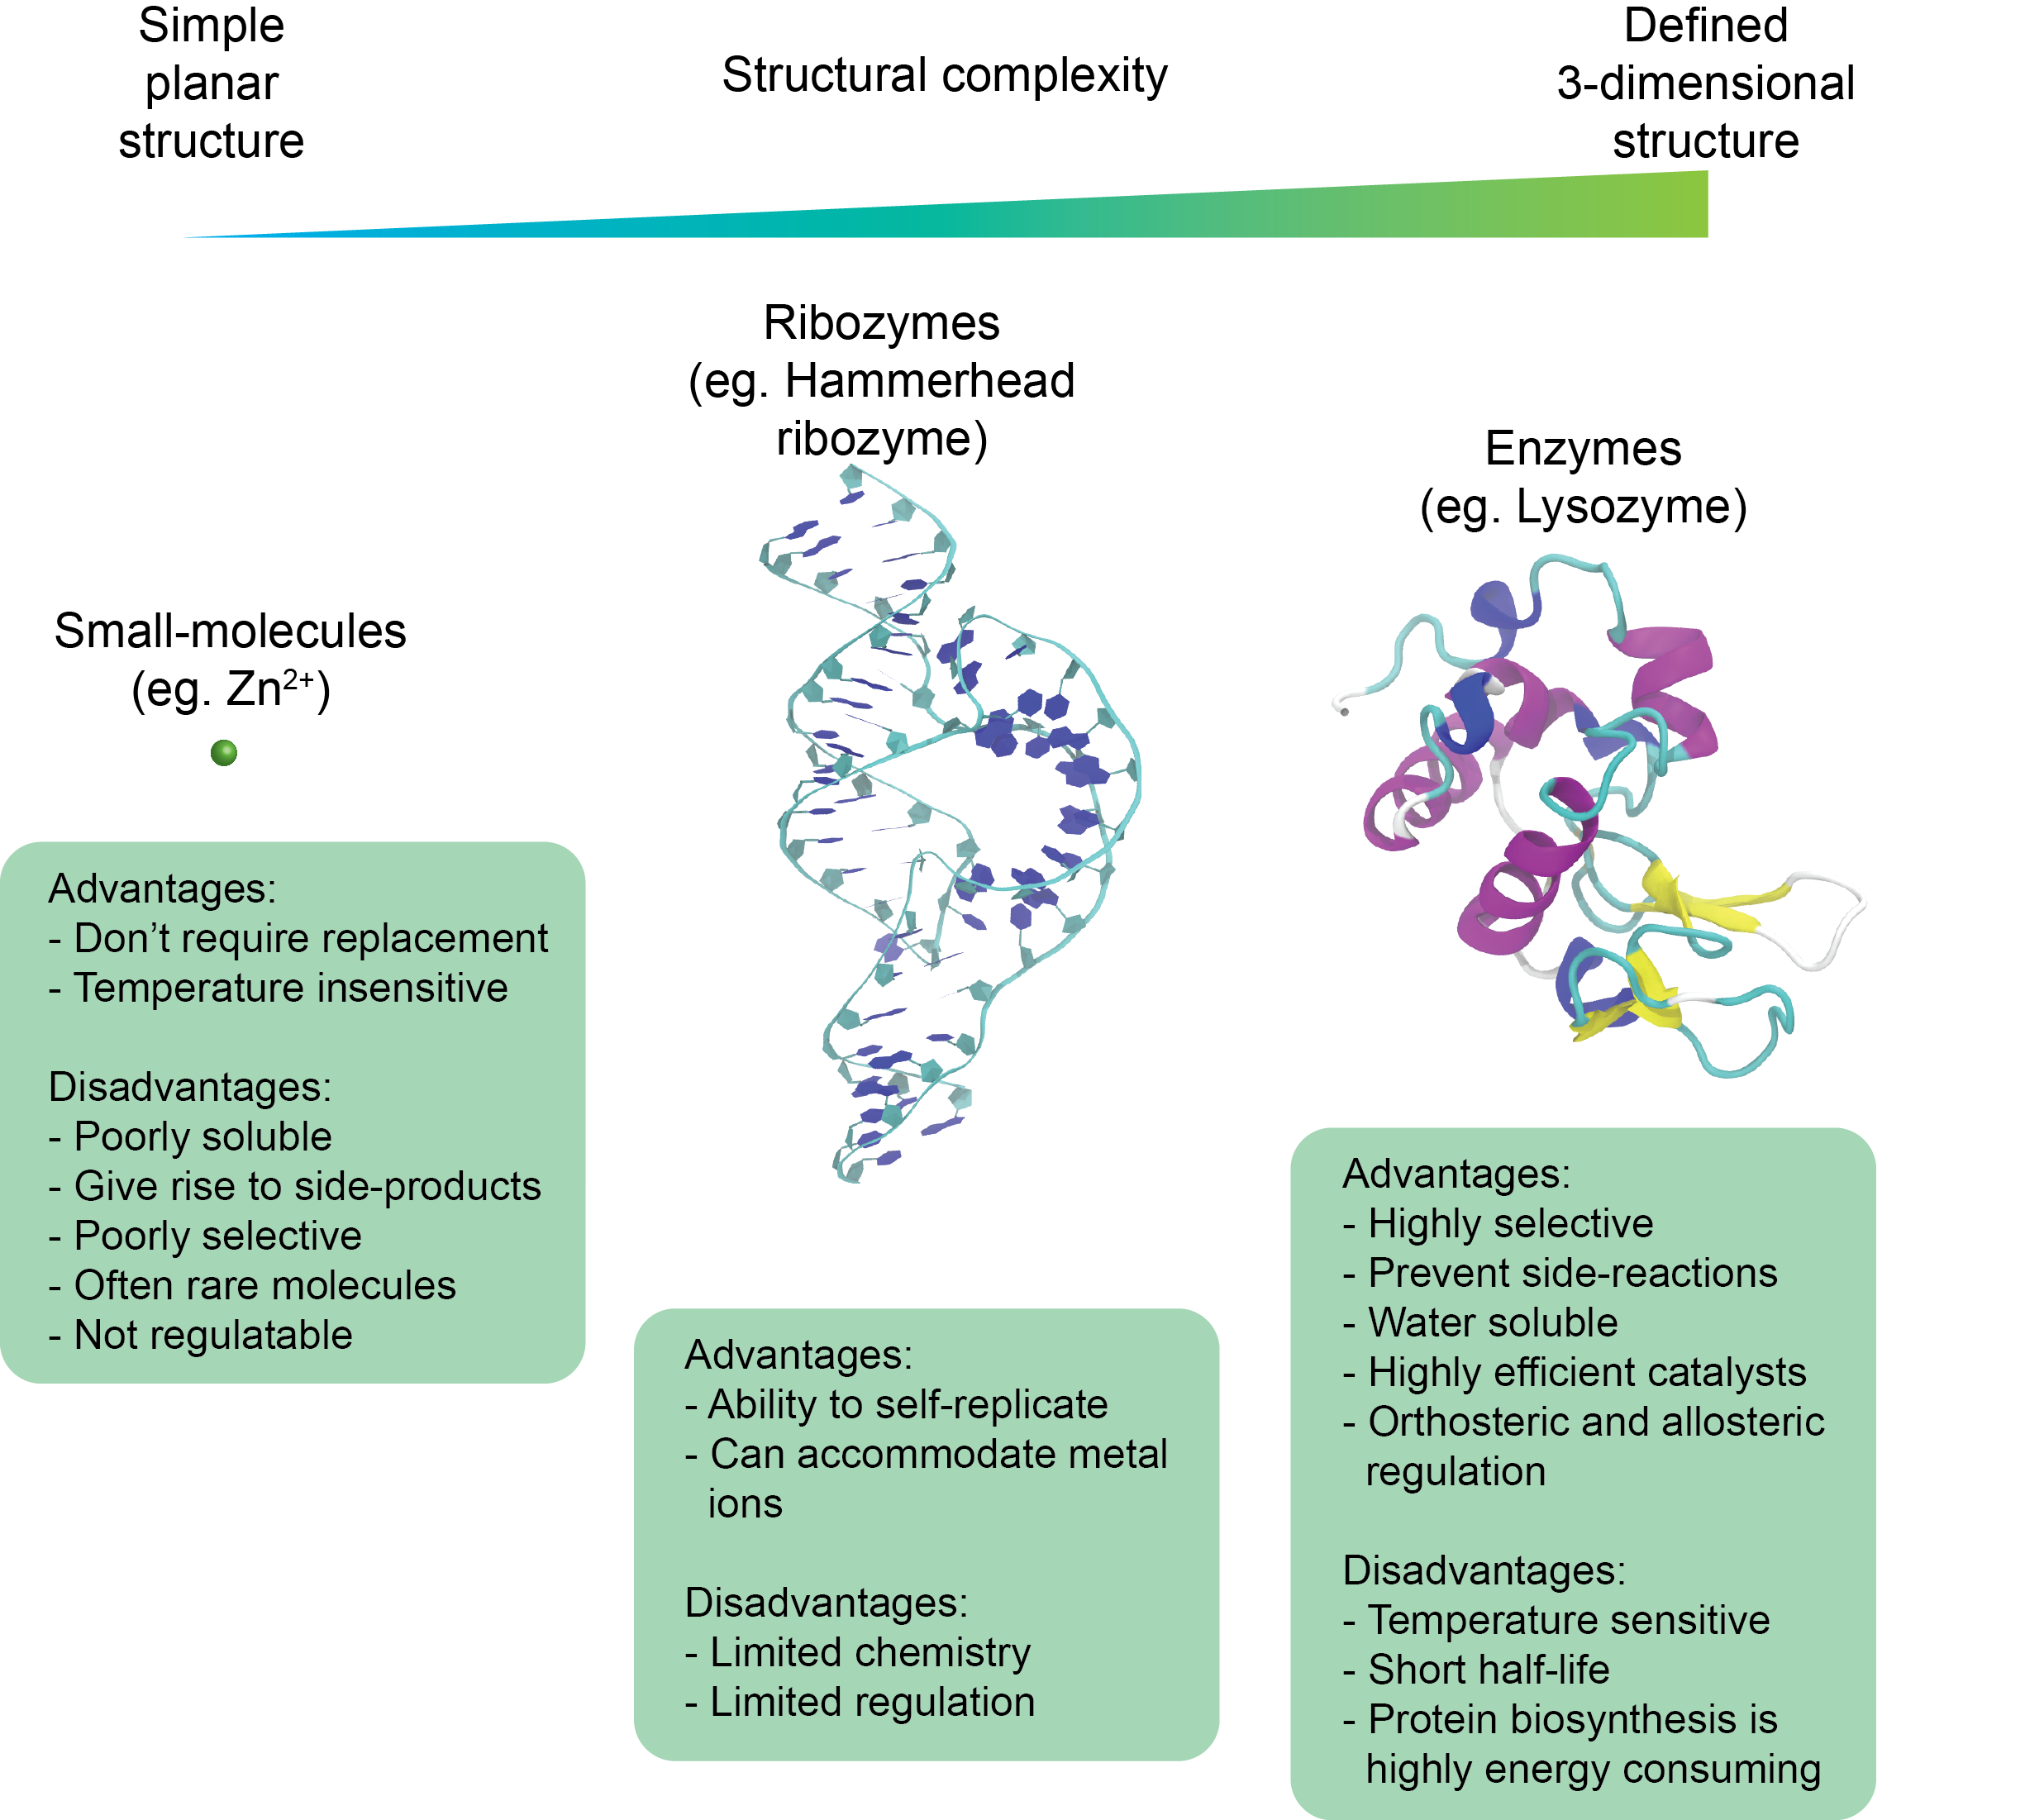
\includegraphics[scale=0.6]{catalysts.png}
\caption[Biological catalysts.]{\textbf{Biological catalysts.} An illustration of the structural complexity of small molecule catalysts, ribozymes and enzymes, and their advantages and limitations.}
\label{fig:biol_catalysts}
\end{figure}
%
%
\clearpage

\subsection{Metabolic homeostasis is maintained by allosteric regulation}

The \textit{in vivo} capacity of an enzyme to realise a particular catalytic flux, at steady-state, is determined by its abundance and kinetic properties. Enzyme abundance can be regulated by gene expression, whereas the kinetic properties of enzyme-catalysed reactions are regulated post-translationally through covalent modifications under the control of signalling pathways and via interactions of enzymes with small molecules. The average concentration of a metabolite in central carbon metabolism is of the order of 1 mM, while glycolytic flux varies between 0.1 and 0.3 (mM$\cdot$ s$^{-1}$).\cite{Tanner:2018aa} Assuming steady-state conditions, where the rate of metabolite production is approximately equal to the rate of consumption, the rate of turnover of the pool of metabolites ($r$) can be determined:
%
%
\begin{equation}
r = \frac{P}{v} \qquad ,where \quad \frac{\partial P}{\partial t} = 0
\end{equation}
%
%
where $P$ is the pool size, $v$ is flux and $t$ is time. The turnover time of metabolites in glycolysis therefore has an approximate range in mammalian cells between 2.8 s and 0.93 s. A quantitative model of time-dependent gene expression changes in mouse fibroblast cells estimated a median transcription rate of approximately 3 mRNAs per hour and and a median translation rate of about 140 proteins per mRNA per hour \cite{Schwanhausser:2011aa}. Therefore, if the reactions of metabolite consumption and production are not in balance, the metabolite pool will become rapidly consumed (or compounded) before gene expression can affect changes to enzyme activity by changing expression levels. Uncontrollable flux imbalances in cells would precipitate an unsustainable biological situation where the metabolite pool would be converted into a handful of compounds, consistent with the end-products of the most energetically favoured enzyme-catalysed reactions in the metabolic network. In essence: metabolism cannot afford to wait for gene expression changes. Instead, the kinetic properties of metabolic enzymes must be tightly regulated to ensure homeostasis.
%
%
\\\\
%
%  
Feedback inhibition in metabolism was first hypothesised by Novick and Szilard (1950) \cite{Novick:1950aa}, when studying the regulation the tryptophan synthesis pathway, and has since been found in almost every biosynthetic pathway. Computational models of simple metabolic networks found that product-feedback inhibition enables optimal growth of cells by minimizing futile cycling and optimizing fluxes \cite{Goyal:2010aa}. Goyal \textit{et al.} (2010) \cite{Goyal:2010aa} showed that, while feedback inhibition is sufficient to control fluxes, the effectiveness of simple product-feedback inhibition comes at the cost of producing high levels of certain metabolite pools, which would likely cause toxicity and osmotic imbalance in cells. Large metabolite pool sizes can be restricted if feedback inhibition is ultra-sensitive. In addition to active (orthosteric) sites, complex enzyme structures present additional \textit{allosteric} binding pockets to which metabolites and other small molecules can bind. Subsequent to binding to an allosteric pocket, information can be propagated over significant biomolecular distances to enact changes to the active site, thereby changing the kinetic properties of the enzyme. This mechanism is known as allosteric regulation and has the potential to both inhibit and activate enzyme activity on very short temporal scales (typically in the range of ns to ms), thus providing a highly sensitive regulatory mechanism for the maintenance of homeostasis. 
%
%
\\\\
%
%
Tight regulation of enzyme catalysis on short timescales is particularly evident in glycolysis, where feed-forward and feed-back regulation manifests in rapidly oscillating concentrations of glycolytic metabolites. This oscillatory behavior of glycolysis was first discovered in yeast cells \cite{Chance:1964aa}. In early investigations, glucose was fed at a continuous rate to yeast cell extracts and oscillations were observed in the concentrations of glycolytic intermediates with a frequency of several minutes \cite{Das:1991aa}. Acute changes to the composition of the extracellular environment also leads to rapid changes in mammalian cell glycolysis, which can be rationalised by enzyme regulation on short temporal scales. Empirical evidence for this hypothesis has been provided recently by studies using fluorescence sensors to monitor the redox balance between nicotinamide adenine dinucleotide in its oxidised (NAD$^{+}$) and its reduced (NADH) forms, as representative of the balance between oxidative and reductive metabolism. Using a genetically-encoded fluorescence peredox sensor, Hung \textit{et al.} (2011) \cite{Hung:2011aa} found that the exchange between cytosolic NADH and NAD$^{+}$ occurred within minutes of acute changes to culture media of mouse neuroblastoma cells, suggesting that glycolytic flux rapidly reaches the steady-state. Taken together, the rapid equilibration of cellular metabolites in response to changed extracellular conditions shows that metabolic homeostasis is maintained on far shorter time scales than can be achieved by gene expression changes, requiring allosteric regulation of enzyme catalysts.
%
%
\\\\
%
%
Due to the importance of allosteric regulation in maintaining homeostatic control of cellular metabolism, subtle changes to the regulation of metabolic enzymes can result in significant alterations to the phenotype of a cell. This is well exemplified in several disease states including cancer, where characteristic changes to central carbon metabolism have been shown to play essential roles in sustaining rapid growth and proliferation. Some pro-tumorigenic features of metabolism can be attributed to changes in gene expression, such as oncogenic mutations in the Ras/Erk pathway resulting in enhanced glucose uptake. Ras-driven over expression of hexokinase-2 in 3T3 cells was shown to lead to increased rates of glycolytic flux, thus increasing the rate of turnover of the metabolite pool by up to 30 \% \cite{Tanner:2018aa}. This introduces a greater requirement of cancer cells for allosteric regulation of metabolic enzymes, to maintain metabolic homeostasis in the context of increased flux. Indeed, many of the changes to metabolic reprogramming in cancer cells have been linked to altered allosteric regulation of key metabolic enzymes. Changes to enzyme regulation is further compounded by aberrant growth factor signalling, which can alter enzyme activity through post-translational covalent modifications, and by changes to nutrient availability in the tumour microenvironment, which can result in changes to intracellular metabolite pools. 

\clearpage

\section{Metabolite-autonomous allosteric regulation of pyruvate kinase}
Mammalian glycolysis involves the conversion of the six-carbon sugar glucose into the three-carbon keto-acid pyruvate, through a series of ten enzyme-catalysed reactions (\textbf{Fig. \ref{fig:pkm2_met_network}}). In addition to providing cellular energy in the form of adenosine triphosphate (ATP) and pyruvate, which can be further oxidised to form acetyl-CoA that enters into the TCA-cycle, glycolytic intermediates also provide precursors for biomass production. Regulation of glycolytic flux plays an important mechanistic role in mammalian physiology, contributing not only to circulating glucose homeostasis and providing ATP, but also to the provision of biomass building blocks in contexts such as cell proliferation, immune activation and angiogenesis. Glucose-utilising pathways are, in turn, coupled to the interconversion of several co-factors including NAD(P)H that contribute to reduction-oxidation homeostasis.
%
%
\\\\
%
%
Regulation of glycolysis is principally achieved through allosteric regulation of several allosteric enzymes including hexokinase (HK), phosphofructokinase (PFK-1) and pyruvate kinase (PK). Pyruvate kinase exists as one of four mammalian isoforms (PKM1, PKM2, PKL and PKR), all of which catalyse the interconversion of PEP and pyruvate in the terminal step of glycolysis. Differential splicing produces L- and R-type PK mRNA from the \textit{pkl} gene. The expression of PKL is limited to liver and some cells of the pancreas, intestine and kidney, and PKR is expressed in erythrocytes. The human pkm gene has 12 exons with either the 9$^{th}$ or the 10$^{th}$ alternatively spliced to generate the PKM1 or PKM2 transcripts, respectively. Both the PKM1 and PKM2 transcripts are identical in length but encode a 56-amino acid region that differs at 22 residues. This localised difference in the primary sequence forms an allosteric pocket in the C-domain of PKM2 to which an activator fructose 1,6-bisphosphate (FBP) can bind.
%
%
\\\\
%
%
In contrast to the M1 isoform, which is thought to be constitutively active in cells \cite{Anastasiou:2012aa}, the catalytic activity of PKM2 can be modulated by several endogenous metabolites that bind to one of two identified allosteric pockets. Allosteric activators include the up-stream glycolytic intermediate FBP \cite{Sparmann:1973aa}; two amino acids L-serine (Ser) \cite{Chaneton:2012aa} and L-histidine (His) \cite{Yuan:2018aa}; and SAICAR \cite{Keller:2012aa}, an intermediate in purine synthesis. Conversely, the enzyme activity of PKM2 can be inhibited L-tryptophan (Trp) \cite{Yuan:2018aa}, L-alanine (Ala) \cite{Yuan:2018aa}, L-phenylalanine (Phe) \cite{Morgan:2013aa}, a phosphotyrosine peptide \cite{Christofk:2008aa} and T$_{3}$ hormone \cite{Kato:1989aa}. Expression of the M2 isoform is dominant in many adult tissues, and is also expressed in healthy proliferative tissues such as embryonic tissue, lymphocytes and intestinal epithelial cells \cite{Dayton:2016ab}. Additionally, PKM2 is highly expressed in tumour cells \cite{Christofk:2008ab}, and the observation that elevated expression of PKM2 correlates with a poor clinical prognosis \cite{Luftner:2000aa,Lu:2016ac} precipitated efforts to inhibit the activity of PKM2 in an attempt to reduce the elevated glycolytic flux seen in many tumours \cite{Chen:2011aa,Vander-Heiden:2010aa}. A landmark study by Christofk \textit{et al.} (2008) \cite{Christofk:2008ab}, however, revealed that PKM2 over-expression could promote metabolic adaptations to nutritional stress in cell culture and increase tumour growth. This led to the prevailing view that lower PK activity, through the enhanced expression and regulation of the M2 isoform, is beneficial for anabolic metabolism and thus for cell proliferation and tumour growth \cite{Vander-Heiden:2011aa,Vander-Heiden:2009aa,Mazurek:2011aa,Israelsen:2015aa,Dayton:2016ab,Jiang:2012aa}.
%
%
%%% FIGURE
%
\begin{figure}[!ht]
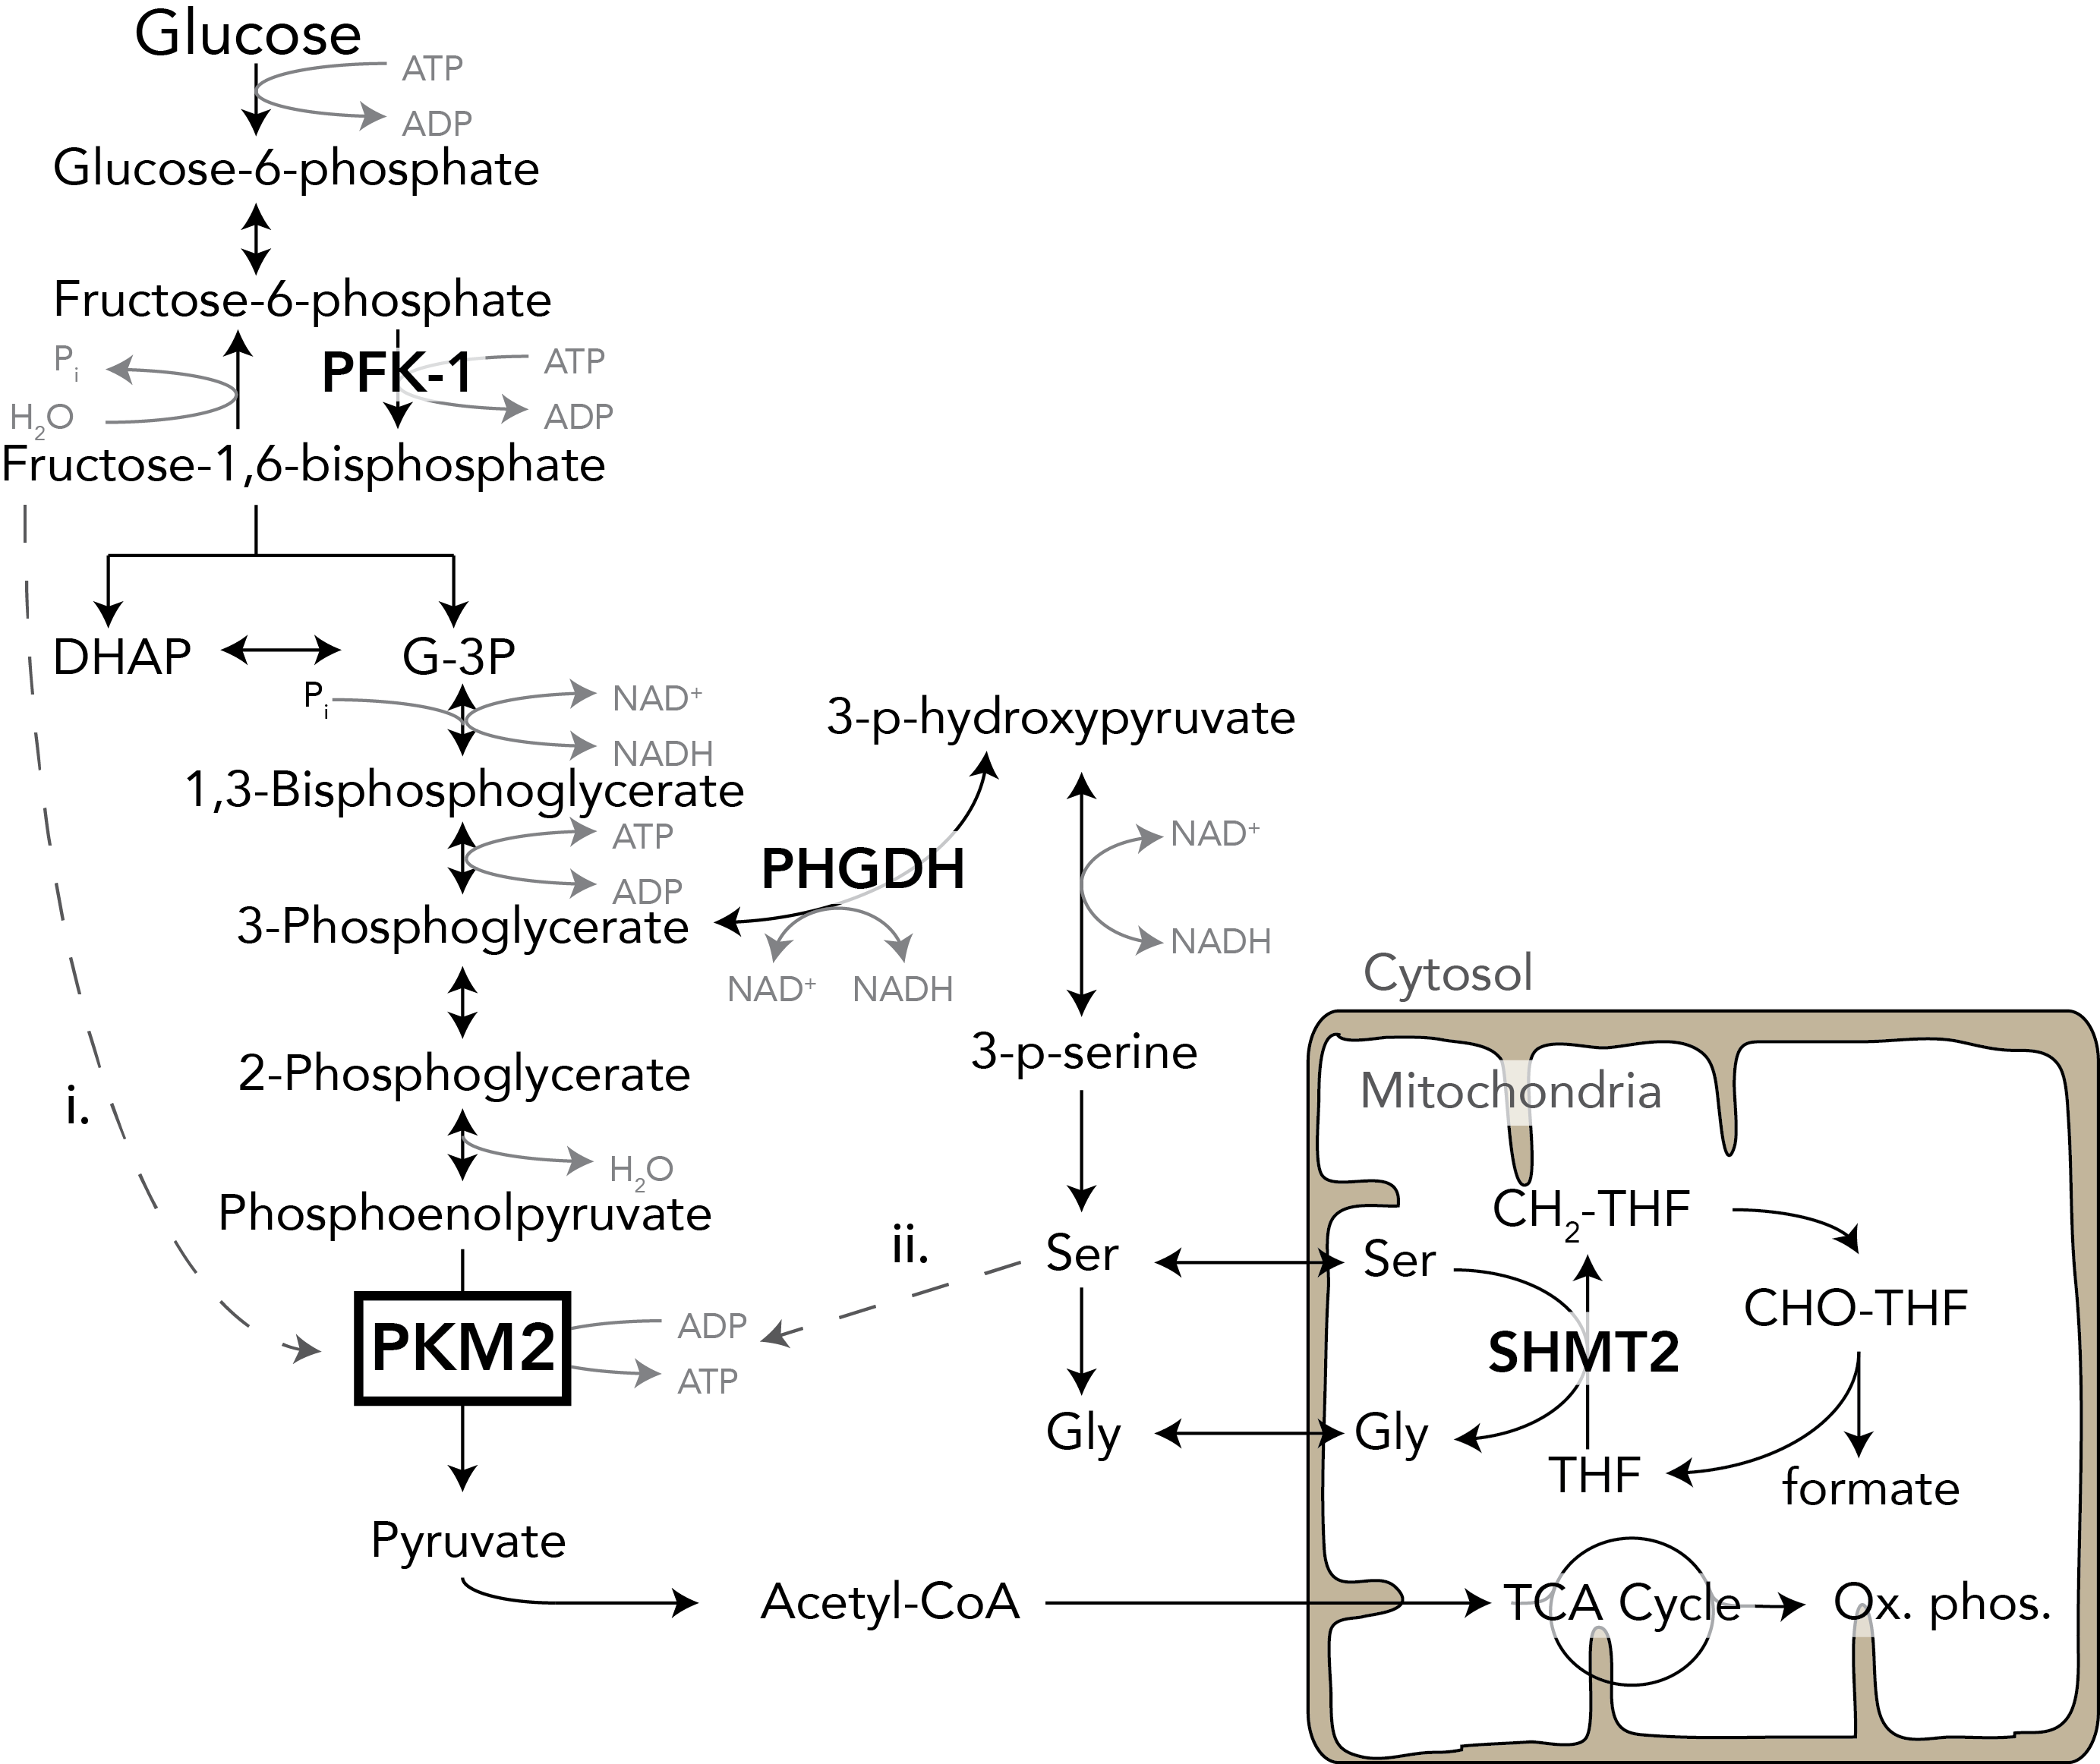
\includegraphics[scale=0.65]{pkm2_met_network.png}
\caption[Allosteric regulation of glucose metabolism.]{\textbf{Allosteric regulation of glucose metabolism.} PKM2 is allosterically regulated by D-fructose-1,6-bisphosphate (FBP; an up-stream glycolytic intermediate) and by L-serine (Ser). Increased glucose uptake results in an accumulation of up-stream glycolytic intermediates. From the current paradigm it follows that accumulation of FBP leads to enhanced allosteric activation of PKM2, through a feed-forward mechanism [i]. Decreased serine uptake due to nutrient deprivation results in reduced binding of serine to PKM2, and hence reduced allosteric activation. This spares glucose carbons for \textit{de novo} serine synthesis and one-carbon metabolism.}
\label{fig:pkm2_met_network}
\end{figure}
%
%

\clearpage

\subsection{Evidence for the involvement of PKM2 regulation in supporting pro-tumourigenic growth}
A number of studies have revealed several mechanisms by which allosteric regulation of PKM2 activity contributes to tumour physiology. \textcolor{red}{Growth-factor signalling pathways have been shown to play a major role in programming metabolic pathways in cells by mediating acute as well as long-term changes in cell metabolism. Activation of protein tyrosine-kinases had previously been shown to result in a decrease in the enzyme activity of PKM2. Christofk \textit{et al.} (2008) \cite{Christofk:2008aa} elucidated the mechanism by which protein-tyrosine kinases acutely regulate the activity of PKM2, finding that aberrant phosphorylation of proteins at tyrosine residues inhibits PKM2 enzyme activity by precipitating the release of the allosteric activator FBP \cite{Christofk:2008aa}. To examine the effect of phosphotyrosine protein binding on FBP-bound PKM2, the authours obtained a peptide binding motif for PKM2 by screening a phosphotyrosine-enriched peptide library matrix to identify novel phosphotyrosine (pTyr)-binding proteins from cell lysates. Christofk \textit{et al.} then synthesized both the phosphorylated and unphosphorylated versions of the optimal peptide: P-M2tide (GGAVDDDpYAQFANGG) and NP-M2tide (GGAVDDDYAQFANGG), respectively for \textit{in vitro} experimentation resembling the domain of a protein tyrosine-kinase with the capacity to bind to PKM2. Moreover, PKM2 inhibition via a signalling-induced protein phosphotyrosine-binding event led to the diversion of glucose carbons away from energy-producing pathways and into lactate and lipid production \cite{Christofk:2008aa}. }
%
%
\\\\
%
%
Additional environmental conditions associated with the tumour microenvironment such as hypoxia, matrix detachment and inflammation can all lead to excess production of reactive oxygen species (ROS) \cite{Halliwell:2007aa,Reuter:2010aa,Schafer:2009aa}, which at sufficiently high concentrations can damage cellular components and compromise cell viability \cite{Wellen:2010aa}. In this context, regulation of PKM2 has been shown to bestow cells with pro-tumourigenic survival advantages. Oxidation of PKM2 at C358 inhibits enzyme activity, promoting the utilisation of glucose carbons through the pentose phosphate pathway to sustain sufficient reducing potential for the detoxification of ROS \cite{Anastasiou:2011aa}. 
%
%
\\\\
%
%
Allosteric inhibition of PKM2 activity can facilitate the utilisation of glucose carbons for \textit{de novo} serine synthesis and one-carbon metabolism. Though generally classified as a nutritionally dispensable amino acid, serine plays an essential role in a number of metabolic processes including the synthesis of other amino acids, lipogenesis and methylation reactions that occur via the generation of S-adenosylmethionine \cite{Yang:2016ab}. Furthermore, the folate cycle, a serine-catabolising process, can regenerate essential cofactors such as NAD(P)H and ATP. As tumour growth supersedes its vascular support, uptake of serine becomes necessary for cancer cell survival. The transfer of human colon cancer cells from culture conditions containing serine to serine-deprived media was found to suppress aerobic glycolysis and enhance the utilisation of glucose carbons in energy producing metabolic pathways \cite{Maddocks:2013aa}. The preference for high-flux aerobic glycolysis in the context of enhanced serine uptake is, in part, driven by allosteric regulation of PKM2. Serine is an allosteric activator of PKM2 \cite{Chaneton:2012aa}, and reduced activation of PKM2 enables cancer cells to adapt to life under limiting nutrient conditions by allowing for the accumulation of glycolytic intermediates, which are subsequently diverted into serine metabolism through phosphoglycerate dehydrogenase (PHGDH). This mechanism ensures that rapidly proliferating cells to sense and respond to availability of serine, thereby retaining a reserve pool of an important biosynthetic precursor. 
%
%
\\\\
%
%
In addition to fluctuations in extracellular concentrations of serine due to limited nutrient supply in poorly vascularised tumors, serine availability can also be limiting due to enhanced activity of enzymes involved in one-carbon metabolism. Rapidly proliferating cancer cells demonstrate an enhanced requirement for nucleotides, resulting from DNA replication stress \cite{Bartkova:2005aa}. Mitochondrial serine hydroxymethyltransferase 2 (SHMT2) catalyses the conversion of serine to glycine, while simultaneously hydrolysing tetrahydrofolate (THF) into 5,10-methylenetetrahydrofolate, a co-factor used in purine biosynthesis (\textbf{Fig. \ref{fig:pkm2_met_network}}). An investigation into the role of serine metabolism within the ischaemic zones of gliomas found that high SHMT2 facilitates a cross-talk between nucleotide biosynthesis and glycolysis by sequestering serine, FBP and SAICAR; thereby reducing oxygen consumption and eliciting a metabolic state that confers a survival advantage to cells in hypoxic tumor regions \cite{Kim:2015aa}. Further in support of this hypothesis, deletion of PKM2 in non-immortalized primary cells from PKM2-conditional mice \cite{Israelsen:2013aa} lead to impaired DNA synthesis and cell cycle progression, resulting from severe thymidine depletion \cite{Lunt:2015aa}. Limiting nucleotide biosynthesis in PKM2-null cells could be rescued by supplementation with exogenous thymidine, suggesting that expression of PKM2, and regulation of its enzyme activity, is required to support DNA synthesis in the context of exponential cell growth \cite{Lunt:2015aa}.
%
%
\\\\
%
%
The mechanistic link between low pyruvate kinase activity and cancer cell proliferation promoted drug-discovery efforts, which identified several small-molecule activators that selectively target PKM2 \cite{Boxer:2010aa,Jiang:2010aa,Walsh:2011aa}. Exogenous PKM2 activators were found to bind to an allosteric pocket, distinct from other binding pockets for FBP and amino acids, and resulted in an increased affinity for the substrate PEP \cite{Anastasiou:2012aa}. An investigation into potential \textit{in vivo} therapeutic effects of the PKM2 activators found that the treatment of mice baring H1299 tumour xenografts with one of the activators Tepp-46, resulted in an inhibition of the xenograft tumors relative to the vehicle-treated control animals \cite{Anastasiou:2012aa}. Impaired tumour growth was accompanied by decreased levels of serine, lactate and ribose phosphate (an intermediate of the pentose phosphate pathway) and increased acetyl-CoA, suggesting that activation of PKM2 resulted in metabolic changes that were incompatible with pro-tumourigenic growth \cite{Anastasiou:2012aa,Kung:2012aa}.
%
%
\\\\
%
%
Taken together, these observations demonstrate that expression of PKM2 affords cancer cells the increased metabolic plasticity to respond to varying environmental conditions that a constitutively high or low activity PK enzyme would not readily allow. Nevertheless, the differential requirements of cancer cell metabolism, and how this is supported by pyruvate kinase expression, remain under investigation. Israelsen \textit{et al.} (2013) \cite{Israelsen:2013aa} generated mice with a conditional allele that abolished PKM2 expression without disrupting PKM1 expression, which were then crossed with a \textit{Brca1}-loss-driven breast cancer mouse model. Intriguingly, mice \textit{without} expression of PKM2 showed an accelerated tumour-associated mortality compared to the wild-type control, suggesting that expression of PKM2 is not required for cancer cell growth and indeed its loss may promote tumour progression under certain conditions. Germline PKM2-\textit{null} mice were found to spontaneously develop multiple macroscopic liver tumours \cite{Dayton:2016aa}. More recently, Morita \textit{et al.} (2018) \cite{Morita:2018aa} reported novel engineered mouse models that express either PKM1 or PKM2, at protein levels equivalent those found endogenously in tissues. The authors found that, across numerous cancer models, expression of PKM1 promoted and PKM2 inihibited tumourigenesis relative to the wild-type control \cite{Morita:2018aa}. 
%
%
\\\\
%
%
The studies by Israelsen \textit{et al.} (2013) \cite{Israelsen:2013aa}, Dayton \textit{et al.} (2016) \cite{Dayton:2016aa} and Morita \textit{et al.} (2018) \cite{Morita:2018aa} highlight a potentially complex relationship between PK expression and cell proliferation. The use of genetic tools to study the role of a metabolic gene in a complex disease are, however, limited in by their binary nature (i.e. comparing a phenotype produced by the knock-out of a single gene with that of wild-type gene expression). In contrast, metabolism, a product of the complex interaction between many genes and the nutritional environment, constitutes a quantitative continuum of phenotypes. Furthermore, spontaneous development of hepatocellular carcinoma in PKM2$^{-/-}$ models is characterised by the depletion of the nucleotides guanosine and cytidine \cite{Dayton:2016aa}, which may suggest impaired DNA replication resulting from decreased glucose utilisation in nucleotide biosynthesis. This, in addition to high systemic inflammation and metabolic changes reported by Dayton \textit{et al.} (2016) \cite{Dayton:2016aa}, may explain why the mice develop tumours in old age. 
%
%
\\\\
%
%
While the metabolic conditions under which PKM2 exerts pro-tumourigenic effects are controversial, allosteric regulation of PKM2 activity remains an important feature of glycolytic control. Crucially, expression of the M2 isoform enables cells to undergo dynamic metabolic changes, which support pro-tumourigenic growth in a number of contexts. Nevertheless, the findings presented by Morita \textit{et al.} (2018) \cite{Morita:2018aa} suggest that the metabolic outcome of cells may not necessarily map to a single enzyme activity status, but rather that both enhanced and decreased pyruvate kinase activity can promote or suppress tumorigenesis, depending on the environment and status of all the other genes in the metabolic network \cite{Allen:2018aa}. Therefore, an understanding of the molecular basis of PKM2 regulation is critical, though this remains largely elusive both in terms of how conformational changes are induced following the binding of allosteric ligands and how PKM2 is able to integrate activating and inhibitory signals after binding to a litany of endogenous allosteric effectors. In this context, the structural and biophysical aspects of PKM2 regulation are reviewed in the following section. 


\clearpage

\subsection{PKM2 protein structure}
Mammalian PKM2 is a homo-tetrameric protein, each protomer containing four structural domains: the A-, B-, C- and N- domains (\textbf{Fig. \ref{fig:pkm2_structure_schematic}}). \textcolor{red}{The protomers within the tetrameric assembly of PKM2 are associated with 222 symmetry. The 222 symmetry is exact only for the A- and C-domains, whereas the B-domains of subunits 1 and 2 are not related to each other by exact two-fold axes because of their different orientations}. The A-domain is the largest of the four, spanning from residues N44 to G116 and P219 to I389, and forms a symmetric $\alpha_{8} \beta_{8}$ TIM barrel. The active site is located within the A-domain, underneath the B-domain cap (\textbf{Fig. \ref{fig:pkm2_structure_schematic}}). The B-domain, consisting of a stretch of residues between P117 and L218 forming eight antiparallel $\beta$-sheets, is mobile and closes on the active site upon binding of the Mg$^{2+}$-ADP substrate complex \cite{Larsen:1998aa}. The C-domain is composed of residues 390-531 and forms five $\alpha$ helices and five $\beta$ sheets. \textcolor{red}{A linear sequence diagram showing the positions of the domains is shown in \textbf{Fig. \ref{fig:pkm2_sequence_schematic}}}. The two-fold symmetry of the homo-tetramer gives rise to two unique protomeric interfaces: the A-A' and the C-C' interfaces. The A-A' interface is formed from the A-domains of two adjacent protomers, consisting of a total of 75 residues with a total surface area of 2.7 nm$^{2}$. There are an estimated 34 hydrogen bonds and 14 salt-bridges that span across the A-A' interface forming contacts between the adjacent protomers. The C-C' interface is less than half the size of the A-A' interface, and is formed of the C-domains of two adjacent protomers in the tetramer assembly, with a total surface area of 1.1 nm$^{2}$. An estimated 17 hydrogen bonds and 11 salt-bridges are formed across the C-C' interface. 
%
%
%%% FIGURE
%
\begin{figure}[!ht]
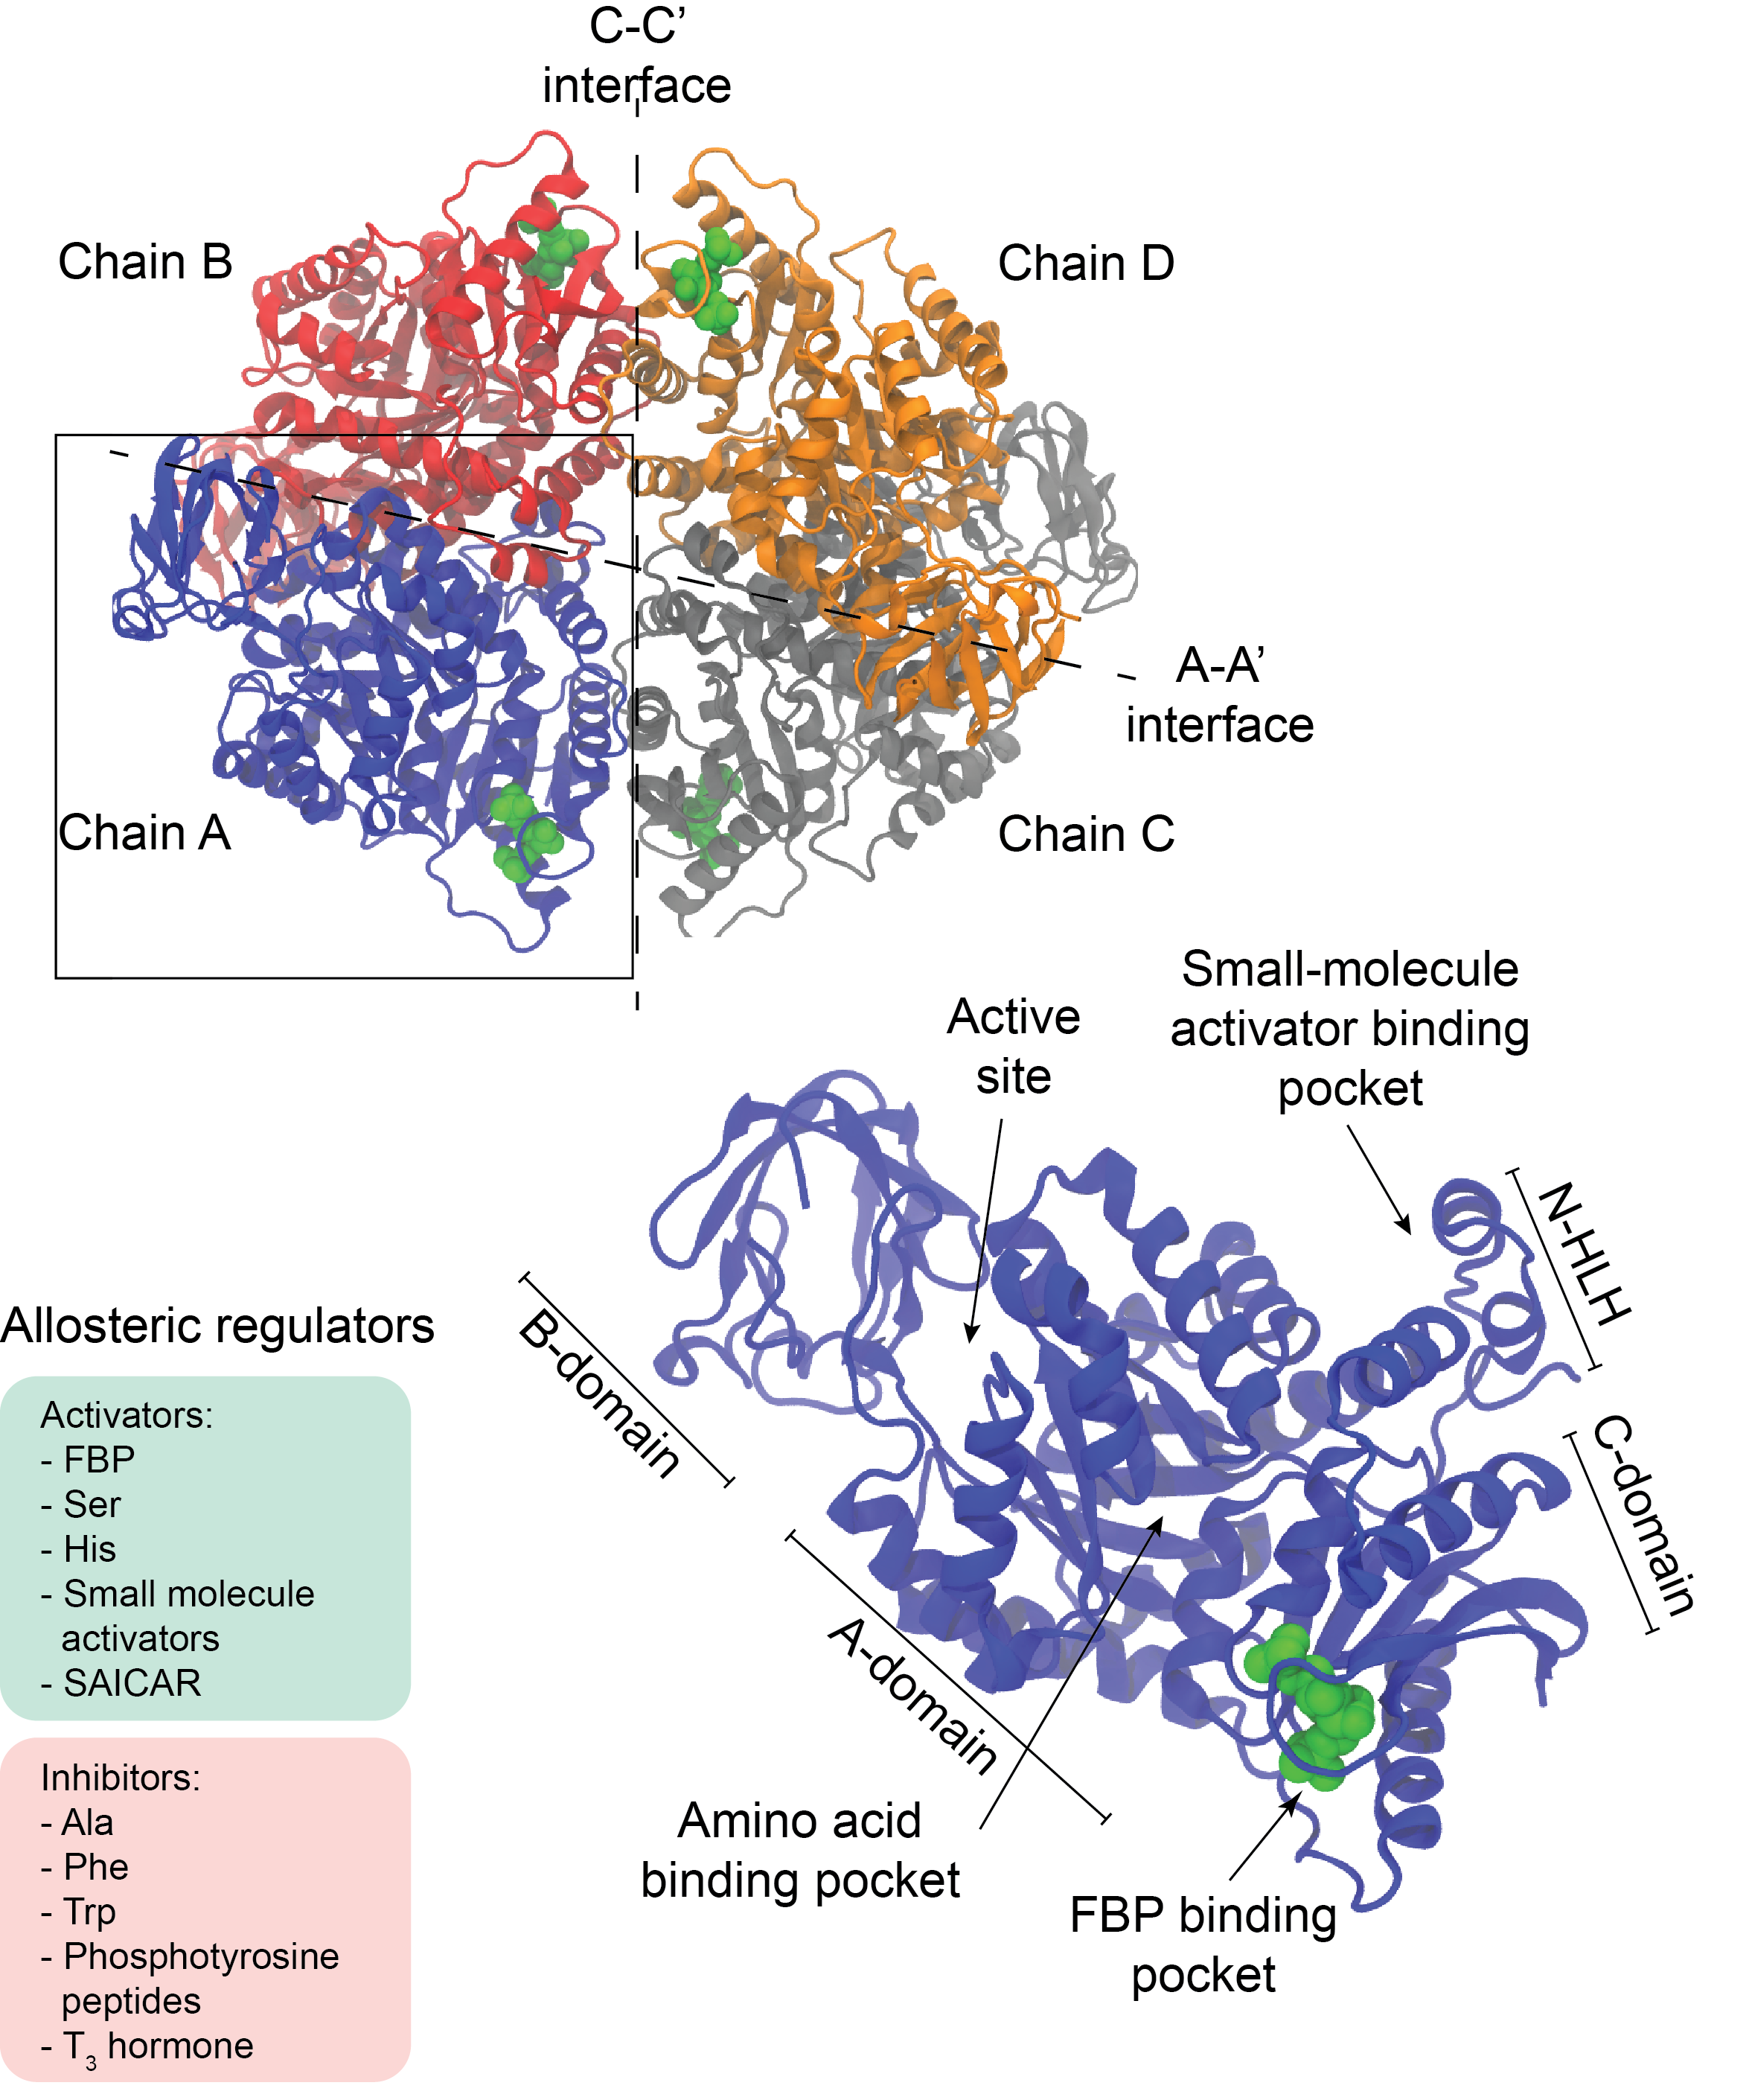
\includegraphics[scale=0.6]{pkm2_structure.png}
\caption[A cartoon representation of the three-dimensional structure of PKM2.]{\textbf{A cartoon representation of the three-dimensional structure of PKM2.} The tetrameric structure of PKM2 is shown above with subunits 1, 2, 3 and 4 of the homotetramer coloured in blue, red, orange and green, respectively. The structure of one of the four monomers within the tetrameric PKM2 complex is shown below. Each PKM2 monomer consists of four structural domains, which are coloured in the cartoon structure. The N-terminal helix-loop-helix is shown in blue, the A-domain is shown in grey, the B-domain is shown in red and the C-domain is shown in green. The C-domain contains the binding pocket for fructose 1,6-bisphosphate, which is shown in an orange space-fill representation. Locations of the active site, the amino acid binding pocket and the small-molecule activator binding pocket are indicated.}
\label{fig:pkm2_structure_schematic}
\end{figure}
%
%
%
%
%%% FIGURE
%
\begin{figure}[!ht]
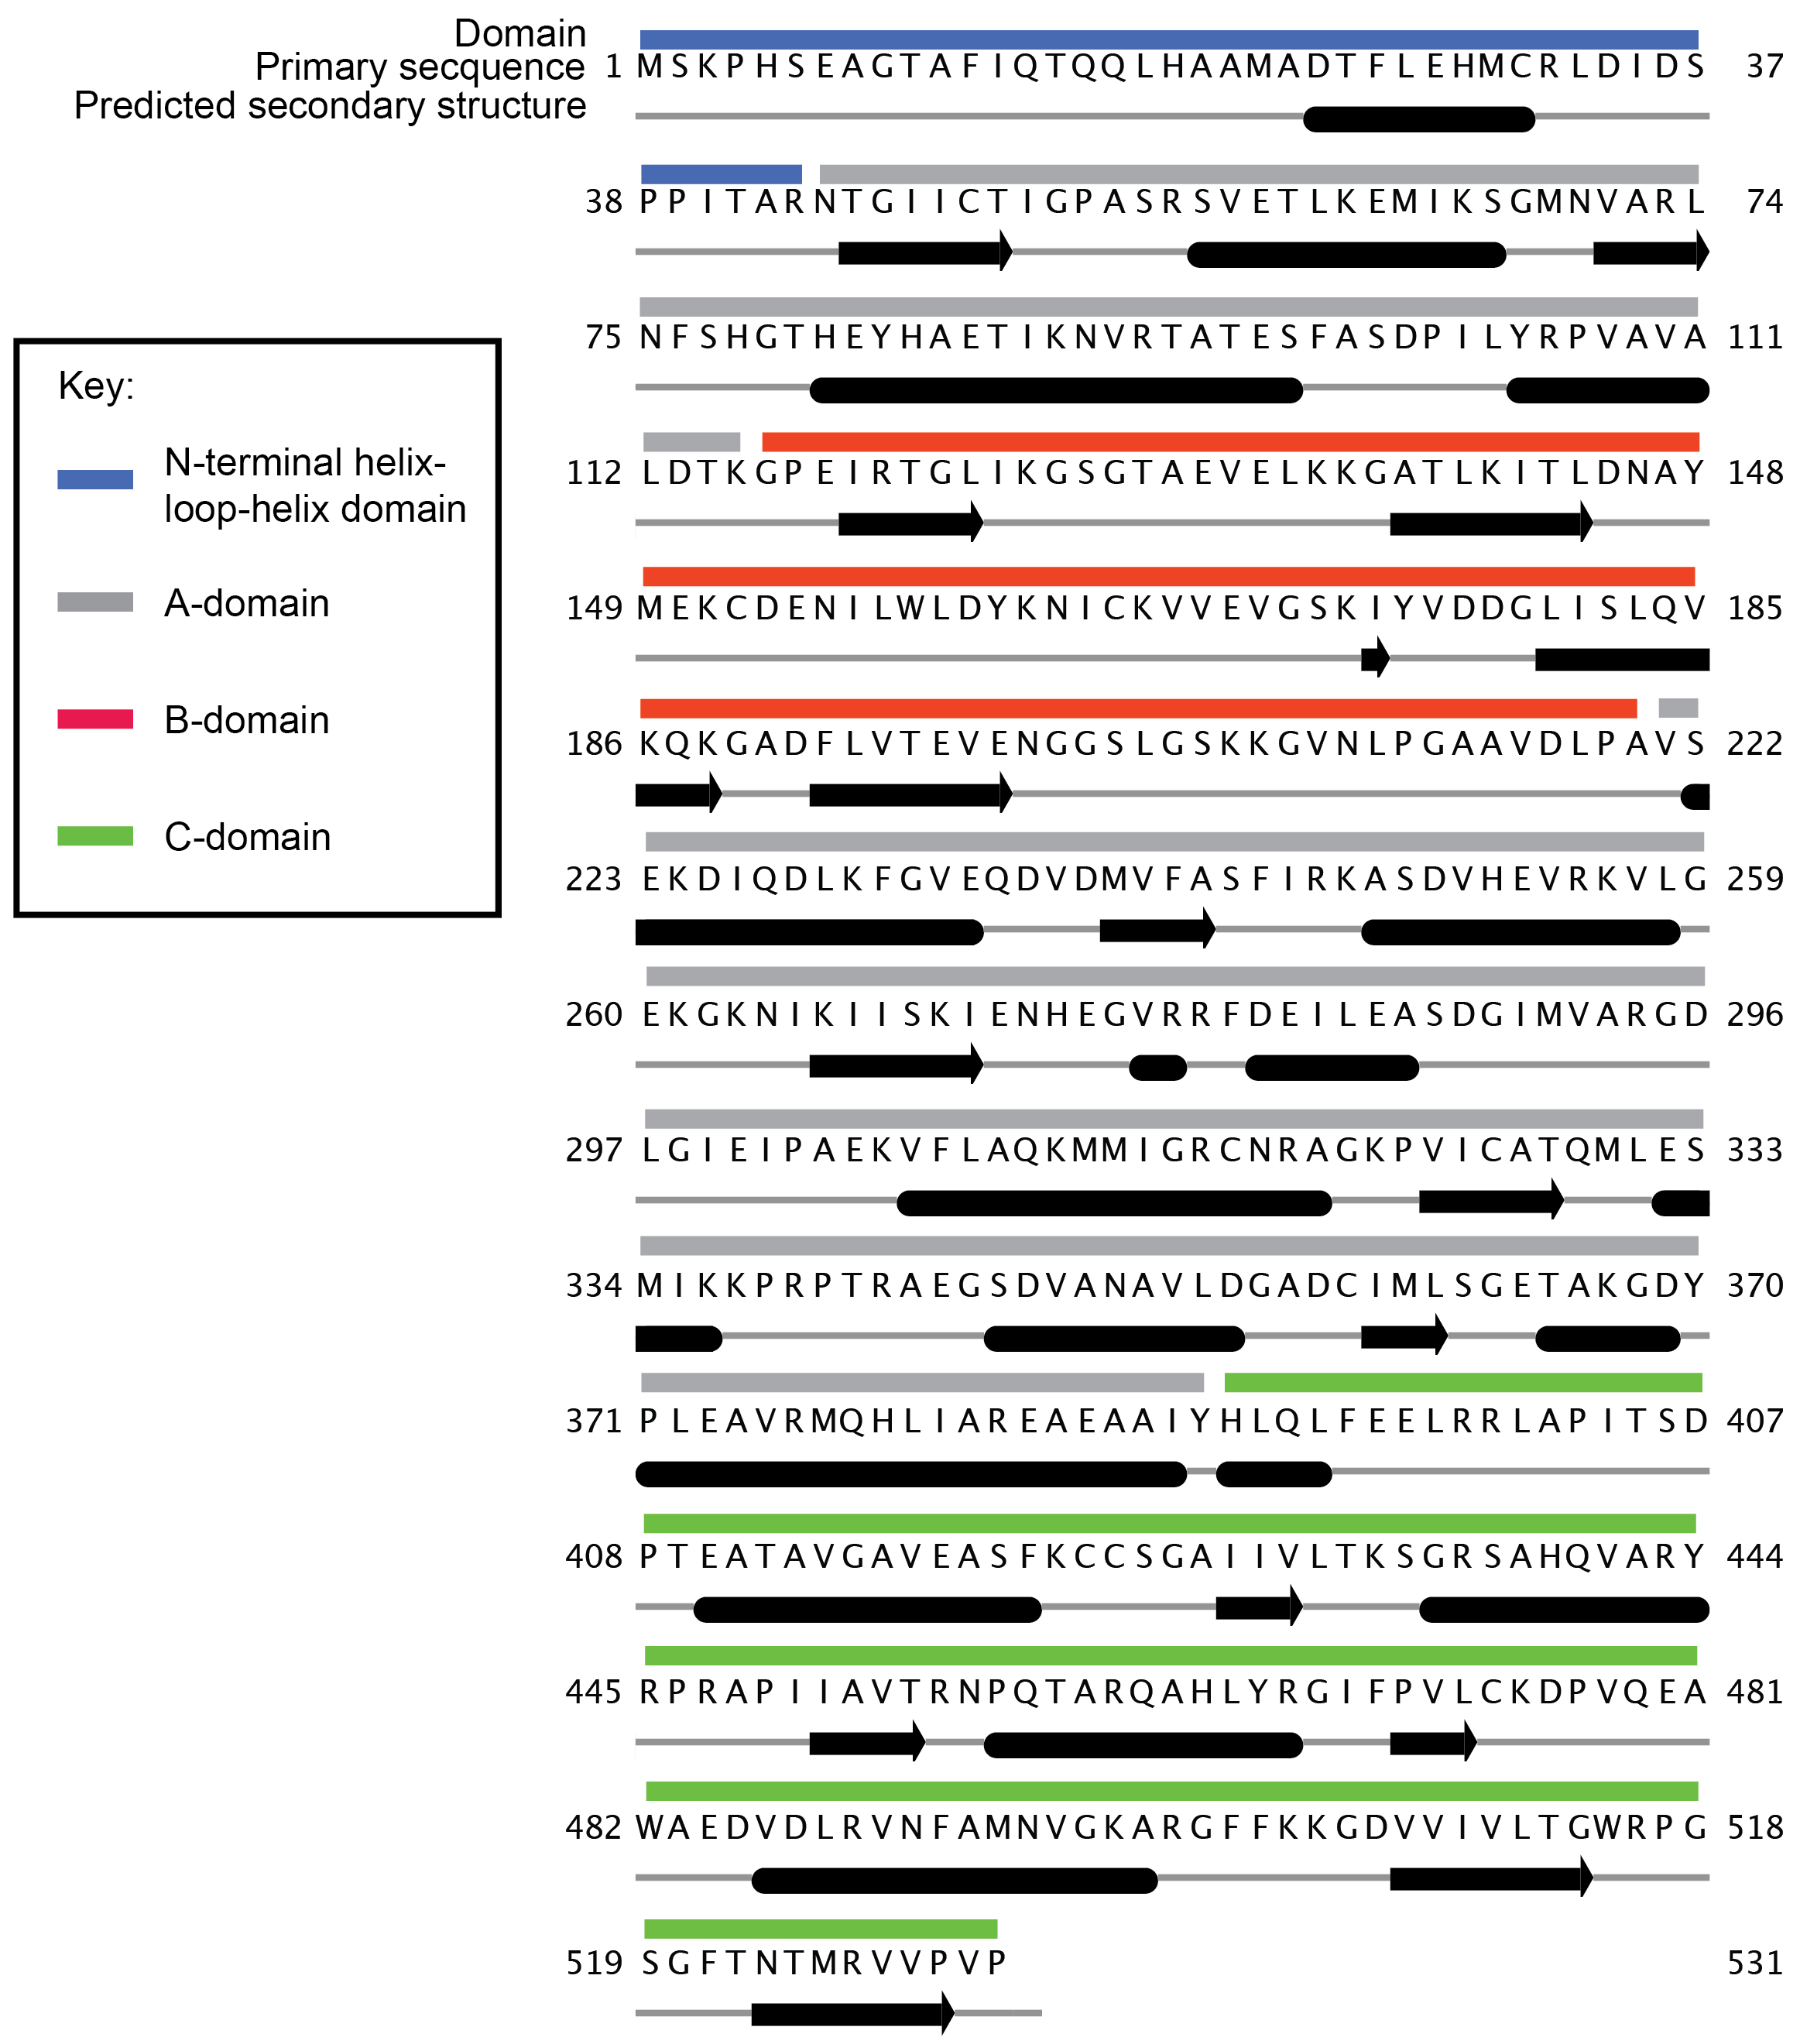
\includegraphics[scale=0.6]{sequence_diagram.png}
\caption[A linear sequence diagram of PKM2.]{\textbf{A linear sequence diagram of PKM2.} The full primary sequence of human PKM2 is annotated with the domain composition and the predicted secondary structure of the protein. The domain composition of the primary sequence is indicated by coloured bars above the protein sequence; the N-terminal helix-loop-helix is indicated with a blue bar, the A-domain with a grey bar, the B-domain with a red bar and the C-domain with a green bar. The predicted secondary structure is shown below the primary sequence; helices are indicated with cylinders and sheets are indicated with thick arrows.}
\label{fig:pkm2_sequence_schematic}
\end{figure}
%
%
%
FBP binds to a pocket within the C-domain of PKM2 (\textbf{Fig. \ref{fig:pkm2_structure_schematic}}), proximal to the C-C' interface and forms interactions with W482, R489, K433, T432, S434, S437, G520 and F521 \cite{Dombrauckas:2005aa}. The N-domain is composed of the first 46 residues in the protein that form a helix-loop-helix, connected to the A-domain by a flexible linker between L33 and G46. The N-domain forms an apolar allosteric pocket to which the small molecule synthetic activators bind, forming contacts with F26, Y390 and L394 \cite{Anastasiou:2012aa}.
%
%
\\\\
%
%
A number of amino acids competitively binding to an allosteric pocket, which is sandwiched between the A- and C-domains \cite{Yuan:2018aa} (\textbf{Fig. \ref{fig:pkm2_structure_schematic}}). Co-crystal structures of PKM2 in complex with either L-histidine (His), L-serine (Ser), L-alanine (Ala), L-tryptophan (Trp) or L-phenylalanine (Phe), found similar binding poses for each ligand \cite{Yuan:2018aa}. All amino acid ligands form charged interactions between their carboxyl-groups and the N$_{\delta}$ group of H464. The diverse side-chain group chemistry of the amino acid ligands is accommodated by a cavernous pocket at the interface between the A- and C-domains.
%
%
%% TABLE
% latex table generated in R 3.4.2 by xtable 1.8-2 package
% 
% latex table generated in R 3.4.2 by xtable 1.8-2 package
% 
\begin{table}[ht]
\begin{tabular}{rlllll}
  \hline
PDB ID & Isoform & Ligands$^{\dagger}$ & Citation \\ 
  \hline
3SRD & M2 & FBP,GOL,K,MG,OXL &  Morgan \textit{et al}. (2013) \cite{Morgan:2013aa} \\ 
3U2Z & M2 & FBP,DZA &  Anastasiou \textit{et al}. (2012) \cite{Anastasiou:2012aa} \\ 
4JPG & M2 & FBP &  Guo \textit{et al}. (2013) \cite{Guo:2013aa} \\ 
4B2D & M2 & FBP,SER &  Chaneton \textit{et al}. (2012) \cite{Chaneton:2012aa} \\ 
4G1N & M2 & MG,NZT,OXL &  Kung \textit{et al}. (2012) \cite{Kung:2012aa} \\ 
4RPP & M2 & FBP &  Wang \textit{et al}. (2015) \cite{Wang:2015aa} \\ 
4QG8 & M2 & GOL,K,MG,MLI &  Wang \textit{et al}. (2015) \cite{Wang:2015aa} \\ 
6B6U & M2 & B3P,CL,K,MG,OXL,PEG,SCN &  Srivastava \textit{et al}. (2017) \cite{Srivastava:2017aa} \\ 
4QGC & M2 & GOL,K,SO4 &  Wang \textit{et al}. (2015) \cite{Wang:2015aa} \\ 
4FXF & M2 &  FBP,K,MG,OXL &  Morgan \textit{et al}. (2013) \cite{Morgan:2013aa} \\ 
4QG9 & M2 &  ACT,MG &  Wang \textit{et al}. (2015) \cite{Wang:2015aa} \\ 
3BJT & M2 & MG,OXL &  Christofk \textit{et al}. (2008) \cite{Christofk:2008aa} \\ 
1T5A & M2 & FBP,GOL,K,MG,OXL,PO4 &  Dombrauckas \textit{et al}. (2005) \cite{Dombrauckas:2005aa} \\ 
6GG4 & M2 & CSO,K,PHE,PO4 &  Yuan \textit{et al}. (2018) \cite{Yuan:2018aa}\\ 
3BJF & M2 & FBP,K,MG,OXL &  Christofk \textit{et al}. (2008) \cite{Christofk:2008aa} \\ 
4QG6 & M2 & PRO &  Wang \textit{et al}. (2015) \cite{Wang:2015aa} \\ 
   \hline
\end{tabular}
\caption[Structures of human PKM2 deposited on the Protein Data Bank.]{\textbf{Structures of human PKM2 deposited on the Protein Data Bank.} $^{\dagger}$Ligand acronyms: D-fructose-1,6-bisphosphate (FBP), glycerol (GOL), potassium (K), oxalate (OXL), 1-(2,3-dihydro-1,4-benzodioxin-6-ylsulfonyl)-4-[(4-methoxyphenyl)sulfonyl]piperazine (DZA), L-tartaric acid (TLA), L-serine (SER), N-(4-{[4-(pyrazin-2-yl)piperazin-1-yl]carbonyl}phenyl)quinoline-8-sulfonamide (NZT), magnesium (MG),  chloride (CL), malonate (MLI), pyruvate (PYR), di(hydroxyethyl)ether (PEG), L-phenylalanine (PHE), acetate (ACT), sulfate (SO4), phosphate (PO4), S-hydroxycysteine (CSO), unidentified atom (UNX).}
\end{table}

\clearpage

\subsection{Kinetics of ligand binding and regulation}
Allosteric regulation of PKM2 acts over long distances to affect the affinity of the enzyme for its substrate phosphoenolpyruvate. The \textit{apo}-form of the enzyme is reported to have a Michaelis-Menten constant for PEP ($K_{M}^{PEP}$) of approximately 2.0 mM \cite{Dombrauckas:2005aa,Chaneton:2012aa,Ikeda:1998aa}. Activation of PKM2 by FBP is associated with a decreased $K_{M}^{PEP}$ of 0.2 mM, while the rate of product turnover ($k_{cat}$) remains unchanged \cite{Yacovan:2012aa,Jiang:2010aa,Dombrauckas:2005aa,Chaneton:2012aa}. Some studies, however, have additionally reported an elevated $k_{cat}$ subsequent to FBP binding \cite{Yuan:2018aa,Morgan:2013aa,Akhtar:2009aa} and the reason for this discrepancy remains unresolved. The $K_{M}$ for adenosine diphosphate (ADP; the second substrate) is reported as approximately 0.4 mM and remains unchanged upon allosteric ligand binding \cite{Ikeda:1998aa,Dombrauckas:2005aa,Chaneton:2012aa}.
%
%
\\\\
%
%
The reported apparent binding affinity of PKM2 for FBP varies considerably between 210 nM \cite{Yan:2016aa} and 7.6 $\mu$M \cite{Morgan:2013aa}. Curiously, isothermal titration calorimetry measurements of FBP binding by Yan \textit{et al.} (2016) \cite{Yan:2016aa} found a sub-stoichiometric association of FBP with PKM2, evidenced by an estimated 0.54 binding sites per PKM2 monomer, despite a reported 1.0 stoichiometry found in several FBP-bound PKM2 crystal structures \cite{Anastasiou:2012aa,Chaneton:2012aa,Christofk:2008aa,Dombrauckas:2005aa}. This result could be explained by the finding that purification of recombinant PKM2 from an \textit{E. coli} expression vector is found to have sub-stoichiometric amounts of co-purified FBP despite extensive dialysis \cite{Gavriilidou:2018aa,Christofk:2008aa,Morgan:2013aa}, supporting the notion that FBP binds tightly to PKM2.
%
%
\\\\
%
%
Several amino acids including Ser, His, Phe, Ala, Trp, Val and Pro have been shown to regulate the activity of PKM2, though the reported effects of the amino acids on PKM2 enzyme kinetic constants vary. Eigenbrodt \textit{et al.} (1983) \cite{Eigenbrodt:1983aa} first showed that PKM2 was susceptible to pronounced activation by Ser and inhibition by Ala, achieved through a positive or negative effect on the enzyme's affinity for its substrate PEP. More recently, Chaneton \textit{et al.} (2012) \cite{Chaneton:2012aa} reported the binding mode for Ser in the amino acid allosteric pocket with an apparent affinity of 810 $\mu$M, acting to decrease the $K_{M}^{PEP}$ from 1.9 mM to 0.19 mM in the absence and in the presence of saturating amounts of Ser, respectively. Taken together, this led to the prevailing view that amino acids act as K-type effectors, and that the rate of product turnover does not change upon ligand binding. Nevertheless, a recent contradictory study, reporting four co-crystal structures of PKM2 bound to Ser, Phe, Trp or Ala, purported to show that amino acids have effects on the $k_{cat}$ \cite{Yuan:2018aa}. 
%
%
\\\\
%
%
In addition to the effects of individual ligands on PKM2 activity \textit{per se}, the multiplicity of distinct allosteric binding pockets on the surface of PKM2 may facilitate concurrent binding of ligands. Therefore, changes to PKM2 enzyme activity are exerted through changes in the concentrations of the metabolite ligands that regulate PKM2. Physical and temporal compartmentalisation of these metabolites may necessitate that PKM2 only responds to specific stimuli, however, it is likely that at any given time several ligands are available to bind to and regulate PKM2.  

\subsection{Concurrent regulation of PKM2 activity by multiple ligands}
PKM2 can bind to multiple allosteric ligands \textit{in vitro} that might either reciprocally influence each other's action, or exert independent effects on enzyme activity. Yet, very little is reportedly known about how PKM2 responds to the simultaneous binding of multiple ligands. A single-point mutation at the FBP binding pocket S473Y prevents FBP binding, though this mutant variant can still be activated by Ser \cite{Chaneton:2012aa}. Conversely, H464A abolishes Ser binding but can be activated by FBP \cite{Chaneton:2012aa}, suggesting that Ser activation could work independently from FBP activation. Inhibitory amino acids that bind to the same pocket as Ser, however, fail to inhibit enzyme activity in the presence of FBP \cite{Yuan:2018aa,Sparmann:1973aa}. The apparent dominant effect of FBP activation may suggest that inhibition by amino acids is blocked by FBP binding, through the promotion of an alternate conformation, or that FBP reduces the binding affinities of the amino acids through a cross-talk between the two binding pockets. Similarly, FBP binding can overcome the inhibition of PKM2 by T$_{3}$ by sequestering PKM2 away from the monomeric species, to which T$_{3}$ binds \cite{Kato:1989aa,Ashizawa:1991aa}. 
%
%
\\\\
%
%
An alternative explaination for how PKM2 is able to integrate multiple regulatory ligands is, rather than a competitive response, through a synergistic response. This might manifest as two activators (eg. FBP and Ser binding) resulting in supra-activated enzyme activity, or alternatively, an activator and an inhibitor displaying a complex non-competitive kinetic phenotype. In support of the latter, Ashizawa \textit{et al.} (1991) \cite{Ashizawa:1991aa} found that FBP addition altered the inhibition of PKM2 activity by Ala, producing only a 30 \% inhibition compared to a 97 \% inhibition of activity in the absence of FBP. Positive synergism has been experimentally found not to occur between Ser and FBP, and between SAICAR and FBP \cite{Keller:2012aa,Chaneton:2012aa}. Interestingly, Zhong \textit{et al.} (2017) \cite{Zhong:2017aa} recently reported that adenosine monophosphate (AMP) and glucose-6-phosphate (G6P) synergistically activate \textit{M. tuberculosis} pyruvate kinase. The authors found that binding of G6P increased the apparent affinity of the protein for AMP, and conversely, that AMP binding increased the binding affinity of G6P \cite{Zhong:2017aa}. While the binding of AMP occurs at a pocket equivalent to that of human PKM2 for FBP, G6P binds to a different pocket that is also distinct from the equivalent amino acid interaction site on human PKM2, and it is intriguing to speculate whether a similar cooperative mechanism occurs between FBP and amino acid binding to human PKM2. Moreover, a recent modelling study purportedly found a synergistic effect of concurrent FBP and Ser binding \cite{Yang:2016aa}. The authors performed molecular dynamics simulations of monomeric PKM2 and found that the predicted free energy of binding to the substrate PEP changed from -48 kJ/mol (either FBP or Ser bound) to -57 kJ/mol (FBP and Ser). Nevertheless, the free energies reported by Yang \textit{et al.} (2016) \cite{Yang:2016aa} translate into a substrate binding affinity of between 10$^{-42}$ M$^{-1}$ and 10$^{-35}$ M$^{-1}$ - a very significant departure from the reported experimental substrate affinity of 1.5 mM. The question of whether binding of allosteric ligands promotes a synergistic effect, therefore, remains unresolved.
%
%
\\\\
%
%
The problem of how PKM2 is concurrently regulated is particularly pertinent in an intracellular context, where multiple allosteric ligands co-exist at varying concentrations and bind to PKM2 with a range of affinities. Notably, the intracellular concentrations of the PK catalytic substrate PEP measured in human colorectal carcinoma cells is less than 10 $\mu$M and only accumulates to 80 $\mu$M upon stable silencing of both PKM1 and PKM2 expression \cite{Chaneton:2012aa}. Low intracellular substrate concentrations suggest that the substrate is limiting for the catalysed conversion into pyruvate. Moreover, the intracellular concentration of FBP has been reported as $\simeq$ 0.5 mM across a panel of cancer cell lines \cite{Xie:2016aa}, which would represent a 2500-fold excess relative to the reported 200 nM binding affinity to PKM2 \cite{Yan:2016aa}. Taken together, evidence from the existing literature suggests that concurrent binding of multiple allosteric ligands may be feasible under certain cellular metabolic conditions, and that there is a selective pressure towards a significant fraction of PKM2 remaining constitutively bound to FBP in order to sustain flux through the PK reaction, which is reported to be high relative to other rate-limiting enzymes in glycolysis \cite{Shestov:2014aa}. Therefore, the interaction between PKM2 and its various allosteric ligands warrants further investigation in order to discern the detailed molecular mechanisms involved in the regulation of this complex glycolytic node, with roles in supporting cancer cell proliferation. 
%
%
\\\\
%
%
\begin{tcolorbox}
\textbf{Question 1:} To what extent do cellular metabolic conditions exist under which PKM2 is likely to be bound to multiple allosteric effectors? And how are the effects of concurrently bound ligands, with opposing functional signals, integrated by PKM2 to regulate enzyme catalysis?
\end{tcolorbox}
%

\subsection{Regulation of PKM2 structure and oligomerisation}
PKM2 molecules form in an equilibrium of monomers and tetramers, with some studies reporting the existence of dimers \cite{Yan:2016aa,Hofmann:1975aa,Gavriilidou:2018aa}, in which the tetramer has high enzymatic activity whereas monomers and dimers display basal activity \cite{Ashizawa:1990aa}. Many of the PKM2 allosteric ligands have been shown to modulate PKM2 activity by changing the equilibrium between the monomer, dimer and tetramer. The binding of FBP promotes, whereas T$_{3}$ prevents, tetramerisation \cite{Ashizawa:1990aa,Anastasiou:2012aa,Gavriilidou:2018aa,Morgan:2013aa,Yan:2016aa}. The effect of amino acids on the monomer-dimer-tetramer equilibrium, however, remains controversial. Some reports suggest that Ala promotes the formation of inactive PKM2 dimers \cite{Hofmann:1975aa,Sparmann:1973aa}, whereas others have shown that inhibition by Phe, Ala and Trp stabilises an inactive T-state tetramer by forming hydrogen bonds with the carbonyl oxygen atom from R43, and thus repelling the N-terminal helix-loop-helix \cite{Morgan:2013aa,Yuan:2018aa}. 
%
%
\\\\
%
%
In addition to ligand-dependent oligomerization, evidence suggests that allosteric ligand binding promotes subtle conformational changes within the tetramer. Crystal structures of \textit{L. mexicana} and \textit{T. cruzi} pyruvate kinase isoforms revealed a rigid-body rocking motion of the A- and C-domains, reorienting them within the tetramer, in the T- to R-state transition \cite{Morgan:2010aa,Morgan:2014aa,Naithani:2015aa}. Hydrogen-deuterium exchange experiments reported an increase in global flexibility in \textit{E. coli} type 1 pyruvate kinase upon binding of FBP, and proposed that destabilisation of $\beta$-strands within the TIM-barrel core resulted from ligand binding \cite{Donovan:2016aa}. Further attempts to gain insights into the dynamic mechanism of human PKM2 and \textit{M. tuberculosis} pyruvate kinase regulation, found that allosteric activator binding causes R342 on the A$\alpha$6-helix to reach across the A-A' interface of the tetramer, forming a stabilising hydrogen bound with the backbone carbonyl group of G271 on the adjacent protomer \cite{Zhong:2017aa,Morgan:2013aa}.
%
%
\\\\
%
%
Ligand-induced conformational changes are likely to be limited to subtle backbone changes and side-chain motions, evidenced by the lack of FBP-driven changes to the radius of gyration of human PKM2 tetramers in small-angle X-ray scattering experiments \cite{Yan:2016aa}. A whole-protein mutagenesis study of the human liver isoform of pyruvate kinase (PKL) reported by Tan and Fenton (2017) \cite{Tang:2017aa}, found that approximately 30 \% of residues, when mutated to alanine, perturbed allosteric activation by FBP. The authors concluded that a significant proportion of the protein contributes to allosteric regulation. In the same study, Tan and Fenton (2017) \cite{Tang:2017aa} found that perturbing mutations were dispersed across the structure, rather than localised to domain-domain boundaries, suggesting that large scale domain reorientations are not exclusive to the allosteric mechanism of PKL. 
%
%
\\\\
%
%
The relative contributions of tetramerisation and local structural changes to the mechanism of allosteric activation is disputed. Molecular dynamics simulations of human PKM2 and \textit{L. mexicana} pyruvate kinase have revealed that allosteric activation by D-fructose-1,6-bisphosphate (human) and D-fructose-2,6-bisphosphate (\textit{L. mexicana}) result in the closure of the B-domain over the active site \cite{Naithani:2015aa,Gehrig:2017aa}, consistent with flexible A/ B - inter-domain motions reported in the crystal structure \cite{Srivastava:2017aa,Dombrauckas:2005aa}. The observation by Gehrig \textit{et al.} (2017) \cite{Gehrig:2017aa} that FBP binding recapitulates some of the experimentally described dynamic changes to the structure, within the monomeric species, argues that the \textit{allosteric content} of the protein is encapsulated within the protomeric unit. Christofk \textit{et al.} (2008) \cite{Christofk:2008aa} published the first atomic structure of human PKM2 in the \textit{apo}-form, showing that ligand binding is not required for tetramer formation. It is not clear, however, whether apo-tetramer formation is an artefact of the high protein concentration used for crystallisation (80 mg/mL), as polymer self-assembly is inherently a concentration-dependent process. Moreover, PKM2 has been shown to form a mixture of oligomeric states, in solution \cite{Morgan:2013aa} and in the gas phase \cite{Gavriilidou:2018aa}, though since FBP is known to remain bound to preparations of purified recombinant PKM2, and it is unclear whether the observed tetramers are simply a result of residual FBP.
%
%
\\\\
%
%
The apparent dichotomy between protomer-specific conformational and oligomeric effects of allosteric ligand binding on PKM2 activation raises important and fundamental questions about the structural basis of its regulation. In addition to allosteric effectors, covalent post-translational modifications (PTMs) have been suggested to influence the oligomerisation of PKM2 protomers \cite{Anastasiou:2011aa,Christofk:2008aa}, although the effects of PTMs on the enzyme mechanism remain elusive. Nevertheless, PKM2 activity in cells is frequently inferred from the oligomeric state that the protein is found to adopt \cite{Wang:2017ab,Wang:2017aa,Qi:2017aa,Lim:2016aa,Hitosugi:2009aa,Christofk:2008ab,Anastasiou:2012aa,Anastasiou:2011aa}. Collectively, current evidence suggests that a link between enzyme activity and the oligomeric state exists and, while not well understood, it may play a role in PKM2 regulation. 
%
%
\\\\
%
%
\begin{tcolorbox}
\textbf{Question 2:} What are the contributions of ligand-induced conformational and oligomeric changes to PKM2, and what are the relationships between these allosteric effects and PKM2 activity?	
\end{tcolorbox}
%
%
Many of the current insights into metabolic dependencies in cancer are derived from analyses of developed tumours and so it is unclear whether observed metabolic changes reflect late adaptive events, or a cumulative agglomeration of metabolic adaptations that have been gradually emerging depending on the needs of cancer cells along the various stages of tumour development \cite{Macpherson:2017aa}. Nevertheless, PKM2, and other allosterically regulated metabolic proteins with roles in disease progression, show that genome-encoded and therefore stably propagated metabolic changes in tumourigenesis are potentiated through protein allostery \cite{Macpherson:2017aa}. Therefore, metabolic flexibility may confer advantages suitable for surviving the varying extracellular conditions cancer cells are subjected to during tumourigenesis, so tools that aid the identification of such mechanisms could hold significant power for discovery.


\clearpage


\section{Investigating the role of protein dynamics in allosteric regulation}
Characterising allosteric mechanisms of enzyme regulation offers several advantages for therapeutic interference with the metabolism of cancer cells. Despite the importance of allostery in regulating numerous aspects of cellular physiology, the investigation of the underlying mechanisms remains a challenge for conventional structural approaches and therefore necessitates multi-disciplinary strategies. A critical obstacle in characterising protein allosteric mechanisms is the inherent flexibility of protein structures, which can result in the emergence of latent allosteric pockets \cite{Keedy:2018aa,Bowman:2015aa}. Once an allosteric pocket has been identified, understanding how information is propagated the active site is confounded by the involvement of protein structural motions on a variety of time scales \cite{Motlagh:2014aa}. Furthermore, as exemplified in the case of PKM2, many proteins contain several allosteric pockets that facilitate the simultaneous binding of several ligands. Concurrent binding of multiple allosteric ligands can modulate the functional response of a protein through the action of multiple allosteric pathways \cite{Sol:2009aa}. It remains unclear, however, whether such allosteric pathways operate independently, or integrate, either synergistically or antagonistically, to control protein function. 


\subsection{Enzyme regulation can involve structural or vibrational motions}
Static model representations of proteins are so prevalent that it is easy to misconstrue these dynamic machines for rigid aperiodic crystals. In addition to the process of protein-folding where a protein reaches its native state through a funnel of energetic intermediates (\textbf{Fig. \ref{fig:protein_dynamic_landscape} A}), folded proteins are soft materials with a complexity, due to the absence of periodicity conditions, forcing the macromolecule to assume a single unique structure. Folded proteins can adopt a variety of different structural and energetic configurations that give rise to an ensemble of isoenergetic ground states, referred to here as conformational \textit{sub-states} (\textbf{Fig. \ref{fig:protein_dynamic_landscape} B}). The amplitudes of the structural motions are determined by the physical and chemical nature of the transient bonded interactions that are broken and made in the transitions between sub-states, and are characterised by a hierarchy of vibrational and configurational motions (\textbf{Fig. \ref{fig:protein_dynamic_landscape} B}). 
%
%
%%% FIGURE
%
\begin{figure}[!ht]
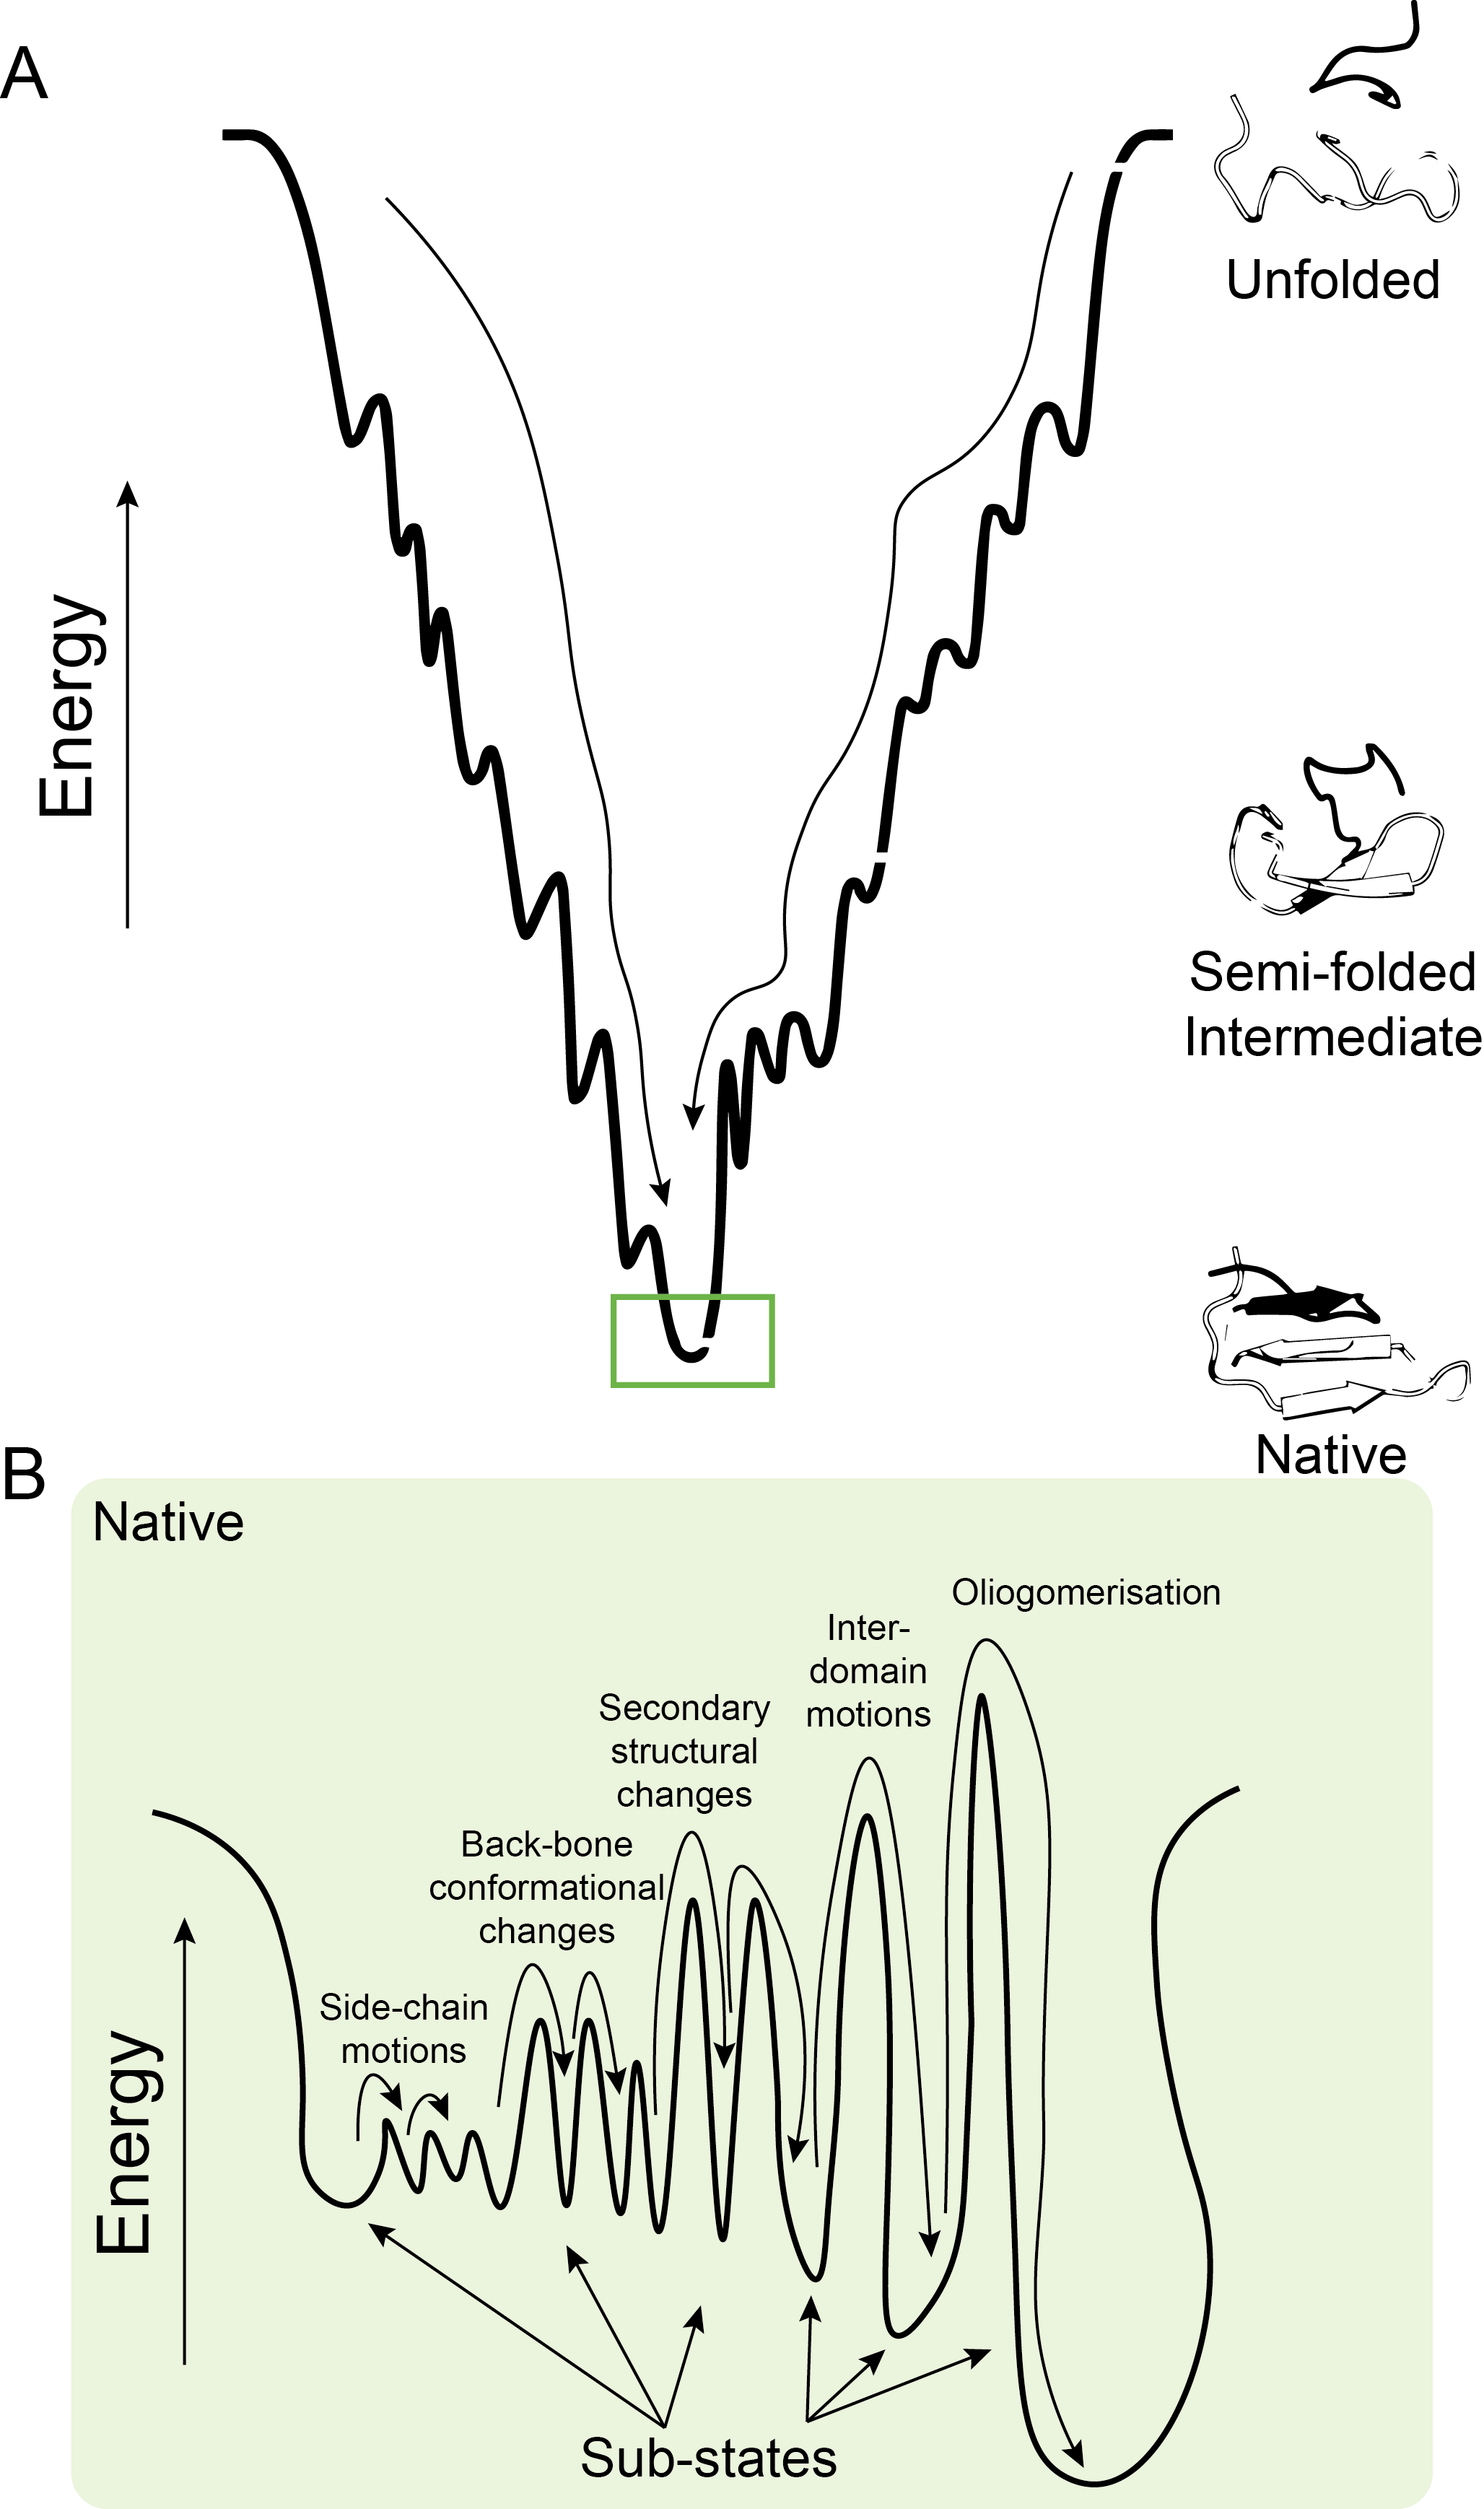
\includegraphics[scale=0.6]{conformational_landscape.png}
\caption[The energetic landscape of protein folding and native protein dynamics.]{\textbf{The energetic landscape of protein folding and native protein dynamics.} \textbf{(A)} A cartoon representation of the energetic landscape of protein folding. \textbf{(B)} The native state of a protein consists of an ensemble of conformations, which are termed conformational sub-states. The transitions between conformational sub-states are characterised by a hierarchy of protein dynamics including (i) side-chain motions, (ii) protein backbone conformational changes, (iii) secondary structural changes (iv) inter-domain motions and (v) oligomerisation of multi-meric proteins. Each respective motion necessitates that the protein overcomes energy barriers, the heights of which are determined by the free energy required for a specified motion.}
\label{fig:protein_dynamic_landscape}
\end{figure}
%
%
%
\clearpage
%
%
Initial evidence for conformational sub-states of a protein came in the early 1970s from measurements of the rate of carbon monoxide (CO) re-association to the heme centre of myoglobin (Mb) following photolysis \cite{Alberding:1976aa,Austin:1973aa,Austin:1975aa}. The first crystal structures published in 1960 by Kendrew \textit{et al.} (1960) \cite{KENDREW:1960aa} had shown that Mb does not have a permanent channel through which CO can exit, suggesting that the exit must proceed through a transient channel caused by dynamic fluctuations of the protein. It was therefore hypothesised that the study of ligand escape from its binding to the heme centre as a function of external parameters such as temperature, pressure and solvent viscosity, would yield information on the fluctuations that underpin the protein dynamics of myoglobin \cite{Frauenfelder:1978aa}.
%
%
\\\\
%
%
In a seminal paper by Austin \textit{et al.} (1975) \cite{Austin:1975aa} the Mb-CO bonded interaction was photolysed with a laser pulse, allowing the CO ligand to migrate within the protein and then finally escape into the bulk solvent. The rate of CO exit ($k_{exit}$) determined over a range of temperatures is plotted in \textbf{Fig. \ref{fig:co_exit_rate}}, along with typical rate constants of fluctuations of bulk solvent ($k_{\beta}$) and fluctuations of the first hydration shell of a solvated protein ($k_{\alpha}$). While the rate of fluctuations in the bulk solvent were found to follow the Arrhenius law, $k_{\alpha}$ and $k_{exit}$ become non-exponential at temperatures $T < 220 K$. This revealed the existence of a glassy state adopted by proteins at very low temperatures, in the absence of protein conformational flexibility. Protein flexibility was found to be restored around 220 K, allowing for an exponential rate of reversible binding of the CO ligand to the heme centre of Mb.
%
%
%%% FIGURE
%
\begin{figure}[!ht]
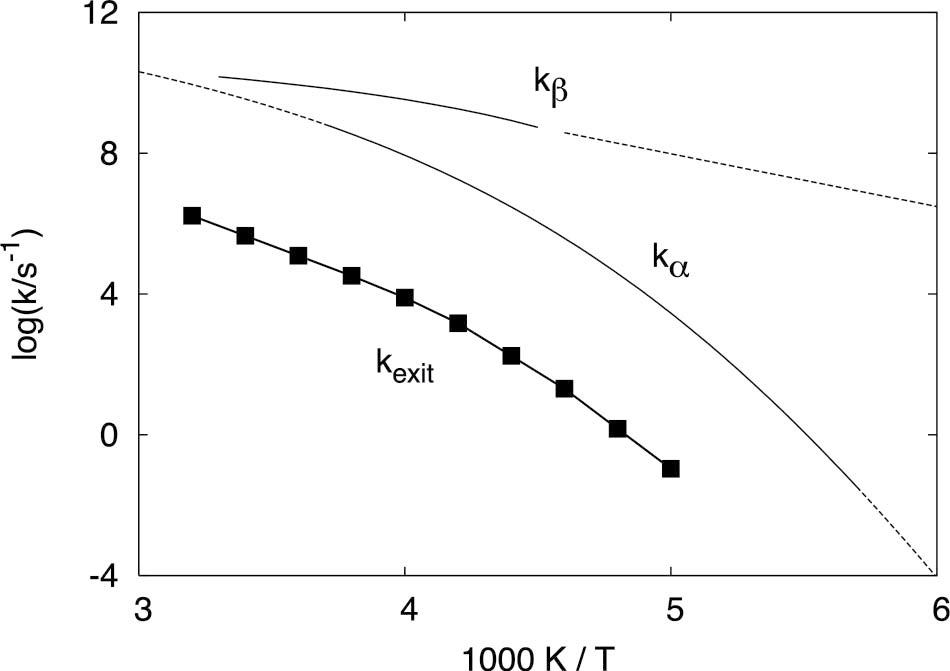
\includegraphics[scale=1]{co_exit_rate.png}
\caption[Typical rate coefficients as a function of temperature.]{\textbf{Typical rate coefficients as a function of temperature.} The rate constant $k_{\beta}$ rate of fluctuations in the bulk solvent, $k_{\alpha}$ is the rate constant of fluctuations in the first hydration shell and $k_{exit}$ is the rate constant of CO exit from myoglobin. All rate constants are determined over a range of temperatures. This figure is reproduced from Figure 4 in Frauenfelder \textit{et al.} (2007) \cite{Frauenfelder:2007aa}.}
\label{fig:co_exit_rate}
\end{figure}
%
%
The transition of solvated proteins from a glass-like to a soft-matter is thought to be coupled with interactions between the protein and hydration water in the first solvation shell. This explains the observation that the rate of fluctuations of the solvation shell ($k_{\alpha}$) undergoes a similar non-exponential to exponential transition around 220 K, as does the rate of CO exit from myoglobin. Subsequent experiments measuring the rate of CO exit under varying solvent compositions, found that the protein must overcome distinct free energy barriers as the CO moves within the protein towards its binding site, providing the first evidence for a hierarchy of protein dynamical motions \cite{Alberding:1976aa,Austin:1973aa,Austin:1975aa}. This theory implied that a molecular system of $N$ components (amino acids) has approximately $e^{N}$ states with energies close to that of the ground state and experiences sizeable fluctuations in its internal energy. 
%
%
\\\\
%
%
Experimental evidence for the existence of multiple protein sub-states prompted the investigation of the structural-basis of protein dynamics by temperature-dependent X-ray crystallography. Two consecutive papers by Artymiuk \textit{et al.} (1979) \cite{Artymiuk:1979aa} and by Frauenfelder \textit{et al.} (1979) \cite{Frauenfelder:1979aa} provided the first direct experimental evidence for the notion that protein adopt dynamic structures. In the former publication, authors computed the mean-squared displacement of backbone atoms within human lysozyme and found that the residue displacements constitute a characteristic rigid-body motion \cite{Artymiuk:1979aa}. Displacements were found to be smaller within the core of the protein and greater on solvent-exposed loops of both lysozyme and myoglobin, due to charge fluctuations in the solvent and the hydration shell \cite{Artymiuk:1979aa}. Moreover, Artymiuk \textit{et al.} (1979) \cite{Artymiuk:1979aa} found that the catalytic pocket underwent a significant conformational change upon substrate binding, concluding that "...protein mobility may play a significant part in biological activity...". 
%
%
\\\\
%
%
Allostery had originated from experiments performed by Changeux and co-workers \cite{CHANGEUX:1961aa,MONOD:1963aa,MONOD:1965aa}, and for decades the two dominant models for allostery were the 'sequential', or KNF (Koshland-Nemethy-Filmer) model \cite{Koshland:1966aa} and the 'symmetric' or MWC (Monod-Wyman-Changeux) model \cite{MONOD:1965aa}, both of which still contribute to the abstraction of complex allosteric mechanisms \cite{Changeux:2013aa}. The two essential features of the MWC model were that an equilibrium was proposed to exist between two conformational states, usually known as the R ('relaxed') and T ('tense') states, in the absence of any ligand, and that symmetry is maintained, so that all subunits in a oligomeric protein change between the R and the T states in a concerted manner \cite{Cornish-Bowden:2014aa}. Conversely, the sequential model did not require conformational symmetry but instead necessitated a strict application of induced fit, with one conformation existing only when the ligand is not bound \cite{Cornish-Bowden:2014aa}. While both the MWC and KNF models agreed on the importance of structural transitions between two pre-defined conformational states whole equilibrium was shifted by the binding of a ligand, both were phenomenological and consequently did not answer the fundamental question of how the binding of a ligand potentiated an allosteric effect at an atomic level of detail \cite{Cui:2008aa}.
%
%
\\\\
%
%
The subsequent accessibility of experimental methods capable of determining protein structure gave rise a stereochemical model of allostery, first proposed by Max Perutz, whereby allostery could be understood in terms of structural changes that could be gleaned through an inspection of high-resolution structures of proteins in the \textit{apo} and \textit{holo} states. In this model, oxygen binding to the T-state triggers the movement of the ferrous iron into the heme plane, realignment of the neighbouring helices and breakage of of inter-subunit salt bridges, thereby shifting the quarternary equilibrium toward the R conformation \cite{Perutz:1970aa}. The elucidation of the initial structures of haemoglobin in two forms (the T- and R-forms) supported the notion that allostery as a general phenomenon might be understood, perhaps in all systems, if only the structures of the allosteric states and the transitions between those states could be determined. Nevertheless, crystal structures are limited in that they provide only a limited snapshot of a single \textit{consensus} conformational state.
%
%
\\\\
%
%
Moreover, despite the fact that plots of estimated mean-square fluctuations versus residue number remain a standard part of the analysis of high-resolution structures, the contribution of overall translation and rotation as well as crystal disorder to B-factors, continues to be a source for concern in their interpretation \cite{Karplus:2002aa}. It was understood that the best means to study the structural basis of cooperativity displayed by haemoglobin, and other allosteric proteins, was to have available a way of calculating the energy of the protein as a function of the atomic positions. To this end, Gelin and Karplus developed a method for calculating the side-chain potentials of bovine peptide tripsin inhibitor (BPTI) using an empirical energy function \cite{Gelin:1975aa}. The same approach was applied towards calculating the forces on the atoms of haemogloblin for the minimisation of its energy in response to ligand binding on the heme group \cite{Gelin:1977aa}, providing the first comprehensive description of distal side-chain motions involved in the transition. 
%
%
\\\\
%
%
Next, Karplus and co-workers used the forces computed from an empirical potential energy function in Newton's equation to simulate protein dynamics, which came to be known as molecular dynamics (MD) simulations. MD simulation methods had already been developed, prior to the 1970s, for simpler systems such as liquid argon with a soft-sphere (Lennard-Jones) potential \cite{Rahman1964aa}, followed by simulations of complex fluids \cite{Stillinger1974aa}. The first MD simulation of bovine peptide tripsin inhibitor (BPTI) \textit{in vacuo} performed by McCammon \textit{et al.} (1977) \cite{McCammon:1977aa}, made clear that proteins are relatively soft polymers and, consequently, have significant structural fluctuations at room temperature; i.e., the static view of the structure of biomolecules had to be replaced by a dynamic picture.
%
%
\\\\
%
%
While allosteric transitions are often accompanied by structural changes, long-range communication between sites can also be mediated by changes in dynamic fluctuations about the mean conformational state (ie. in the absence of structural changes), which are driven by entropic changes in the protein. Dryden and Cooper (1984) \cite{Cooper:1984aa} first proposed that an allosteric effector may simply change the broadness of the free energy basin of the protein conformational state, rather than shifting the basin to a distinctly different region. This provided a plausible model for an entropy-driven allosteric mechanism, in the absence of stereochemical conformational changes. Entropy-driven allosteric mechanisms have since been experimentally described. Popovych \textit{et al.} (2006) \cite{Popovych:2006aa} characterised the negatively cooperative binding of cAMP to dimeric catabolite activator protein (CAP). Two cAMP molecules bind to dimeric CAP with negative cooperativity and function as allosteric effectors by increasing the protein's affinity for DNA. The authors showed that the binding of the first cAMP molecule had minimal effects on the conformation of the second cAMP binding site, but rather that distinct change in protein motions between the two sequential cAMP binding steps results in a large difference in conformational entropy \cite{Popovych:2006aa}. This showed that allostery can be mediated exclusively by vibrational changes, rather than large-scale conformational changes. 


\subsection{Allostery is an ensemble phenomenon}
\label{subsec:allostery_ensemble}
Just as protein folding can be viewed as a landscape of possible conformational states surrounding the \textit{native} (free energy minimum) state, a folded protein has an ensemble of conformational sub-states. According to this statistical framework, all possible conformations of a protein are populated within the ensemble according to their free energies. The free energy landscape of a folded protein can be smooth with many accessible states, rough with only a few states, or somewhere in between \cite{Vendruscolo:2005aa}. Allosteric ligands can effectively remodel the energy landscape of proteins, manifesting as enthalpic and/or entropic redistributions within the available configurational space. Therefore, protein function is not determined purely by its static structure but rather through a redistribution of already existing populations in response to ligand binding. 
%
%
\\\\
%
%
The energy landscape of a folded protein contains a plurality of functional mechanisms and, as such, sub-states within the ensemble can be partitioned into configurations that account for the active and inactive states of the enzyme. Nevertheless, investigating the relationships between protein dynamics, activity and structure is hampered by the difficulty in observing all three characteristics simultaneously. A landmark study by Volkman \textit{et al.} (2001) \cite{Volkman:2001aa}, used nuclear magnetic resonance (NMR) spectroscopy to correlate the structural states of the nitrogen regulatory protein C (NtrC) and its interconversion dynamics directly with its biochemical activity. Phosphorylation of NtrC causes the displacement of several structural elements resulting in the exposure of a hydrophobic patch on one side of the molecule, enabling NtrC dimers to self-associate to form oligomers that regulate the transcriptional activity of a number of genes involved in nitrogen metabolism in enteric bacteria. In order to probe $\mu$s - ms time-scale dynamics, Volkman \textit{et al.} (2001) \cite{Volkman:2001aa} measured the chemical shifts of protein backbone atoms and found that the dynamics of various NtrC mutants correlated with their activity, supporting the idea of a population shift between two pre-existing conformations.
%
%
\\\\
%
%
The propensity of an allosteric transition to stabilise a particular sub-state within the conformational landscape, and hence the probability that a protein will exert a given function, is determined by the free energy barrier between the different sub-states. Indeed, within the boundaries of the protein's primary sequence, the free energy between all of the accessible sub-states constrains the landscape of a protein and encodes the structure and function. Yao \textit{et al.} (2008) \cite{Yao:2008aa} used solution NMR measurements to quantify the free energy of the light-sensitive LOV2 (light, oxygen and voltage) domain-J$\alpha$-helix binding equilibrium following light stimulation. Blue light absorption of the LOV domain induces the formation of a covalent adduct between a conserved cysteine residue in the LOV domain and the C4a carbon of the isoalloxazine ring of FMN, leading to a light-dependent enhancement of phototropin kinase activity. Yao \textit{et al.} (2008) \cite{Yao:2008aa} found that this light-sensitive switch is mediated by an equilibrium between two conformations, determined by the positioning of the J$\alpha$ helix between a bound conformation (dark; inactive) and a dissociated state (lit; active). NMR relaxation experiments found that photo-excitation resulted in a redistribution between the bound-dissociated J$\alpha$ equilibrium from 98:2 in the dark state to 9:91 in the light state, with an associated free energy difference of 3.8 kcal mol$^{-1}$. The authors noted that the free energy barrier of the allosteric transition was small relative to the energy of the blue light photons being absorbed by the flavin chromophore ($\simeq$ 64 kcal mol$^{-1}$). Thus, the bonded and non-bonded interactions that make up the protein core fold are generally modest, suggesting that no single state will necessarily dominate the ensemble. As such allosteric mechanisms are likely to be controlled by statistical equilibria and less deterministic than was suggested by classical discrete-state models. 
%
%
\\\\
%
%
As exemplified by NtrC and LOV2, allosteric regulation of proteins can involve transitions between sub-states with unique physical and biochemical properties. Therefore, the role that structural dynamics of a protein play in biological processes can only be understood by characterizing all thermally accessible protein conformations and their populations. Since the free energy landscape of a folded protein contains many conformational sub-states, any macromolecular observable $A$ can be described as an ensemble average over microscopic sub-states given by:
%
%
\begin{equation}
A = \langle a \rangle_{ensemble} = \frac{1}{N} \sum^{N}_{\lambda = 1} a(x_{\lambda})
\end{equation}
%
%
where $x_{\lambda}$ is the sub-state of the $\lambda$th member of the ensemble. In reality, experimental measurements are made only on a single system and all the microscopic detailed motion is present. As such, one observes an averaged observable over time of the detailed motion, which suppresses the microscopic details. Thus, the time average and the ensemble average should be equivalent:
%
%
\begin{equation}
A = \langle a \rangle_{ensemble} = \displaystyle\lim_{t \to \infty} \frac{1}{t} \int_{0}^{t} dt \: a(x(t))
\end{equation}
%
%
It is often straightforward to determine $\langle a \rangle$ from an experiment, while the underlying distribution of $a(x)$ is experimentally inaccessible since the experiment is a time- and ensemble-average over molecular conformations \cite{Burgi:2001aa}. A common approach to dynamic interpretation of NMR relaxation experimental data is to use NOE data and s$^{2}$ order-parameters as constraints for molecular dynamics simulations to simulate a conformational ensemble in agreement with experimental data \cite{Lindorff-Larsen:2005aa}. Such approaches are limited in their application due to complications in performing measurements in a sufficiently diverse combination of alignment media \cite{Guerry:2013aa}. Nevertheless, molecular dynamics simulations can provide a direct sampling of microscopic sub-states $a(x)$ and, as such, present a powerful tool for investigating allosteric transitions of proteins. 


\subsection{Identification of allosteric pathways from molecular dynamics simulations}
Empirical evidence suggests that subsequent to ligand binding to an allosteric site, a network of residues mediates the communication between the allosteric site and the functional centre of the protein (catalytic pocket in the case of enzymes). Communication across the protein, through so-called allosteric pathways \cite{Sol:2009aa}, is mediated by networks of residues that exhibit spatial and/or temporal correlations. It was therefore hypothesised that measuring correlated motions within a protein structure during allosteric transitions, observed from simulated trajectories of the protein conformational ensemble, would lead to the identification of the residues involved in propagating information along allosteric pathways. 

\subsubsection{Covariance measurements of residue correlation}
Long-range positional correlations were first observed in molecular dynamics simulations of bovine trypsin inhibitor (BTPI) and hen white lysozyme (HEWL) by Huenenberger \textit{et al.} (1995) \cite{Hunenberger:1995aa}. The authors measured correlated motions by computing the normalised covariance matrix of atomic fluctuations, after a superposition of the trajectory to the first frame:
%
%
\begin{equation}
C_{ij} = \sqrt{\frac{\langle x_{i} \cdot x_{j} \rangle}{\langle x_{i}^{2} \rangle \langle x_{j}^{2} \rangle}}
\label{equ:pearson_cor}
\end{equation}
%
%
where $x_{i}$ and $x_{j}$ are the vectorial positional fluctuations of atoms $i$ and $j$, respectively. As noted by Ichiye and Karplus (1991) \cite{Ichiye:1991aa} correlations measured of the form in Equ. \ref{equ:pearson_cor} assumes that $x_{i}$ and $x_{j}$ are co-linear vectors, since $C_{ij}$ depends on the angle between both vectors. Moreover, the use of the covariance matrix implies a Gaussian approximation of the underlying configurational space density, and therefore this approach treats correlations in a quasi-harmonic approximation \cite{Lange:2006aa}. The quasi-harmonic approximation of the Hamiltonian implies that the potential energy surface of a protein is parabolic, which is irreconcilable with empirical findings showing that proteins have an ensemble of conformational sub-states (Section \ref{subsec:allostery_ensemble}). 


\subsubsection{Mutual information}
Rather than measuring co-linear motions, mutual information presents a more physically faithful method for computing correlated motions from protein dynamics. The fluctuations of each atom are considered to have a given distribution, and the correlations between distributions are calculated by the joint probability distribution. The fluctuations of two atoms are considered to be completely independent if their joint probability distribution is equal to their marginal probabilities:
%
%
\begin{equation}
p(\mathbf{x}) = \prod ^{N}_{i=1} p_{i}(x_{i})
\label{equ:uncorrelated}
\end{equation}
%
%
where $p(x)$ is the canonical ensemble density $p(x) = Z^{-1} exp \left( - \frac{1}{k_{B}T} V(x + \langle r \rangle ) \right) $, with partition function $Z$, temperature $T$, Boltzmann constant $k_B$, potential energy $V$ and marginal probability density $p_{i}(x_{i})$. The idea behind this analysis to calculate those correlations that violate Equ. \ref{equ:uncorrelated} using the Shannon mutual information:
%
%
\begin{equation}
I[x_{1}, x_{2}, ..., x_{3N}] = \sum^{3N}_{i=1} H[x_{i}] - H[\mathbf{x}] 
\end{equation}
%
%
where $H$ is the entropy of the random variables defined as: $H[\mathbf{x}] = -\int p(\mathbf{x}) \: log \: p(\mathbf{x}) \: d\mathbf{x}$. Focusing on correlations between pairs of atoms:
%
%
\begin{equation}
I[\mathbf{x_{i}}, \mathbf{x_{j}}] = H[\mathbf{x_i}] + H[\mathbf{x_j}] - H[\mathbf{x_{i}}, \mathbf{x_{j}}] 
\end{equation}
%
%
The mutual information between pairs of fluctuating atoms was first used by Lange and Grubmueller (2006) \cite{Lange:2006aa} to measure correlated motions from molecular dynamics simulations of the B1 domain of G protein and T4 lysozyme. The authors noted that a linear covariant qualification of the covariance matrix missed more than 50 \% of the correlations, attributed to a dependence on mutual orientations of the atomic fluctuations and non-linear correlations that emerged in the dynamics \cite{Lange:2006aa}. As such, linear mutual information between distal protein motions has subsequently emerged as a commonly used method for computed correlated motions \cite{McClendon:2014aa,Gasper:2012aa}, and is not susceptible to the problematic assumptions of covariance measures previously highlighted. 


\subsubsection{Discrete-state mutual information}
\label{subsec:discrete_state_mi}
More recently, the use of mutual information to measure correlated motions that underpin allosteric communication was further developed by Kleinjung, Fraternali, and co-workers \cite{Pandini:2012aa,Pandini:2013aa} using a discrete-state formalism for the mutual information calculation. The authors defined a collection of 24 four-residue fragments, which comprised the so-called M32K25 \textit{structural alphabet} \cite{Pandini:2010aa}. \textcolor{red}{Each fragment provides a simple and explicit description of four successive C$\alpha$ atoms along the backbone of a protein and defined by three internal angles. While limited to describing positions of C$\alpha$ atoms, and not considering other fine-grained features of protein structure, the M32K25} structural alphabet (SA) was effective in encoding the structure of all experimental protein structures deposited in the Protein Data Bank, and could therefore be used as a coarse graining method to define the local orientation of a protein backbone in a simulated ensemble (\textbf{Fig. \ref{fig:sa_encoding_analysis} A}). \textcolor{red}{In this context, the \textit{local orientation} of a protein backbone is defined as the vectorial position of successive C$\alpha$ atoms within a protein structure, which is discretised into overlapping four-residue long segments. Insofar as the M32K25 SA maps the vectorial position of successive C$\alpha$ atoms, and thereby changes to the positions of these segments that result from simulated or experimentally obtained protein dynamics, the detected changes are localised to the affected regions of the protein backbone. This makes the analysis of a molecular dynamics trajectory with the M32K25 SA particularly sensitive to backbone conformational changes (e.g. secondary structure transitions) and rather insensitive to side-chain fluctuations.} Rather than a vectorial definition of atomic fluctuation, the discrete-state mutual information between locally-encoded fragments was computed in order to determine distal correlations across the structure:
%
%
\begin{flalign}
I^{n}(C_i; C_j) = \frac{I(C_i; C_j) - \epsilon (C_i; C_j)}{H(C_i, C_j)}
\label{equ:norm_mutual_information1}
\end{flalign}
%
%
where the columns of the structural fragment alignment are given by $C_i$ and $C_j$, $I(C_i; C_j)$ is the mutual information, $\epsilon(C_i; C_j)$ is the expected finite size error and $H(C_i, C_j)$ is the joint entropy. The mutual information is given by
%
%
 \begin{flalign}
I(C_i; C_j) = \sum \sum p(c_i, c_j) \: log_{2} \: \frac{p(c_i, c_j)}{p(c_i) p(c_j)}
\end{flalign}
%
%
where the two columns in the structural alphabet alignment $C_i$ and $C_j$ are random variables with a joint probability mass function $p(c_i, c_j)$, and marginal probability mass functions $p(c_i)$ and $p(c_j)$. The joint entropy $H(C_i, C_j)$  is defined as
%
%
\begin{flalign}
H(C_i; C_j) = - \sum \sum p(c_i, c_j) \: log_{2} \: p(c_i, c_j)
\label{equ:positional_entropy1}
\end{flalign}
%
%
The discrete mutual information calculated for finite state probabilities can be significantly affected by random and systematic errors. In order to account for this, an error term $ \epsilon (C_i; C_j)$ was subtracted from the mutual information $I(C_i; C_j)$ in Equ. \ref{equ:norm_mutual_information1} given by
%
%
\begin{flalign}
\epsilon (C_i; C_j) = \frac{B^*_{C_i C_j} - B^*_{C_i} - B^*_{C_j} + 1}{2N}
\end{flalign}
%
%
where $N$ is the sample size and $B^*_{C_i C_j}$, $B^*_{C_i}$ and $B^*_{C_j}$ are the number of states with non-zero probabilities for $C_i C_j$, $C_i$ and $C_j$, respectively.
%
%
%%% FIGURE
%
\begin{figure}[!ht]
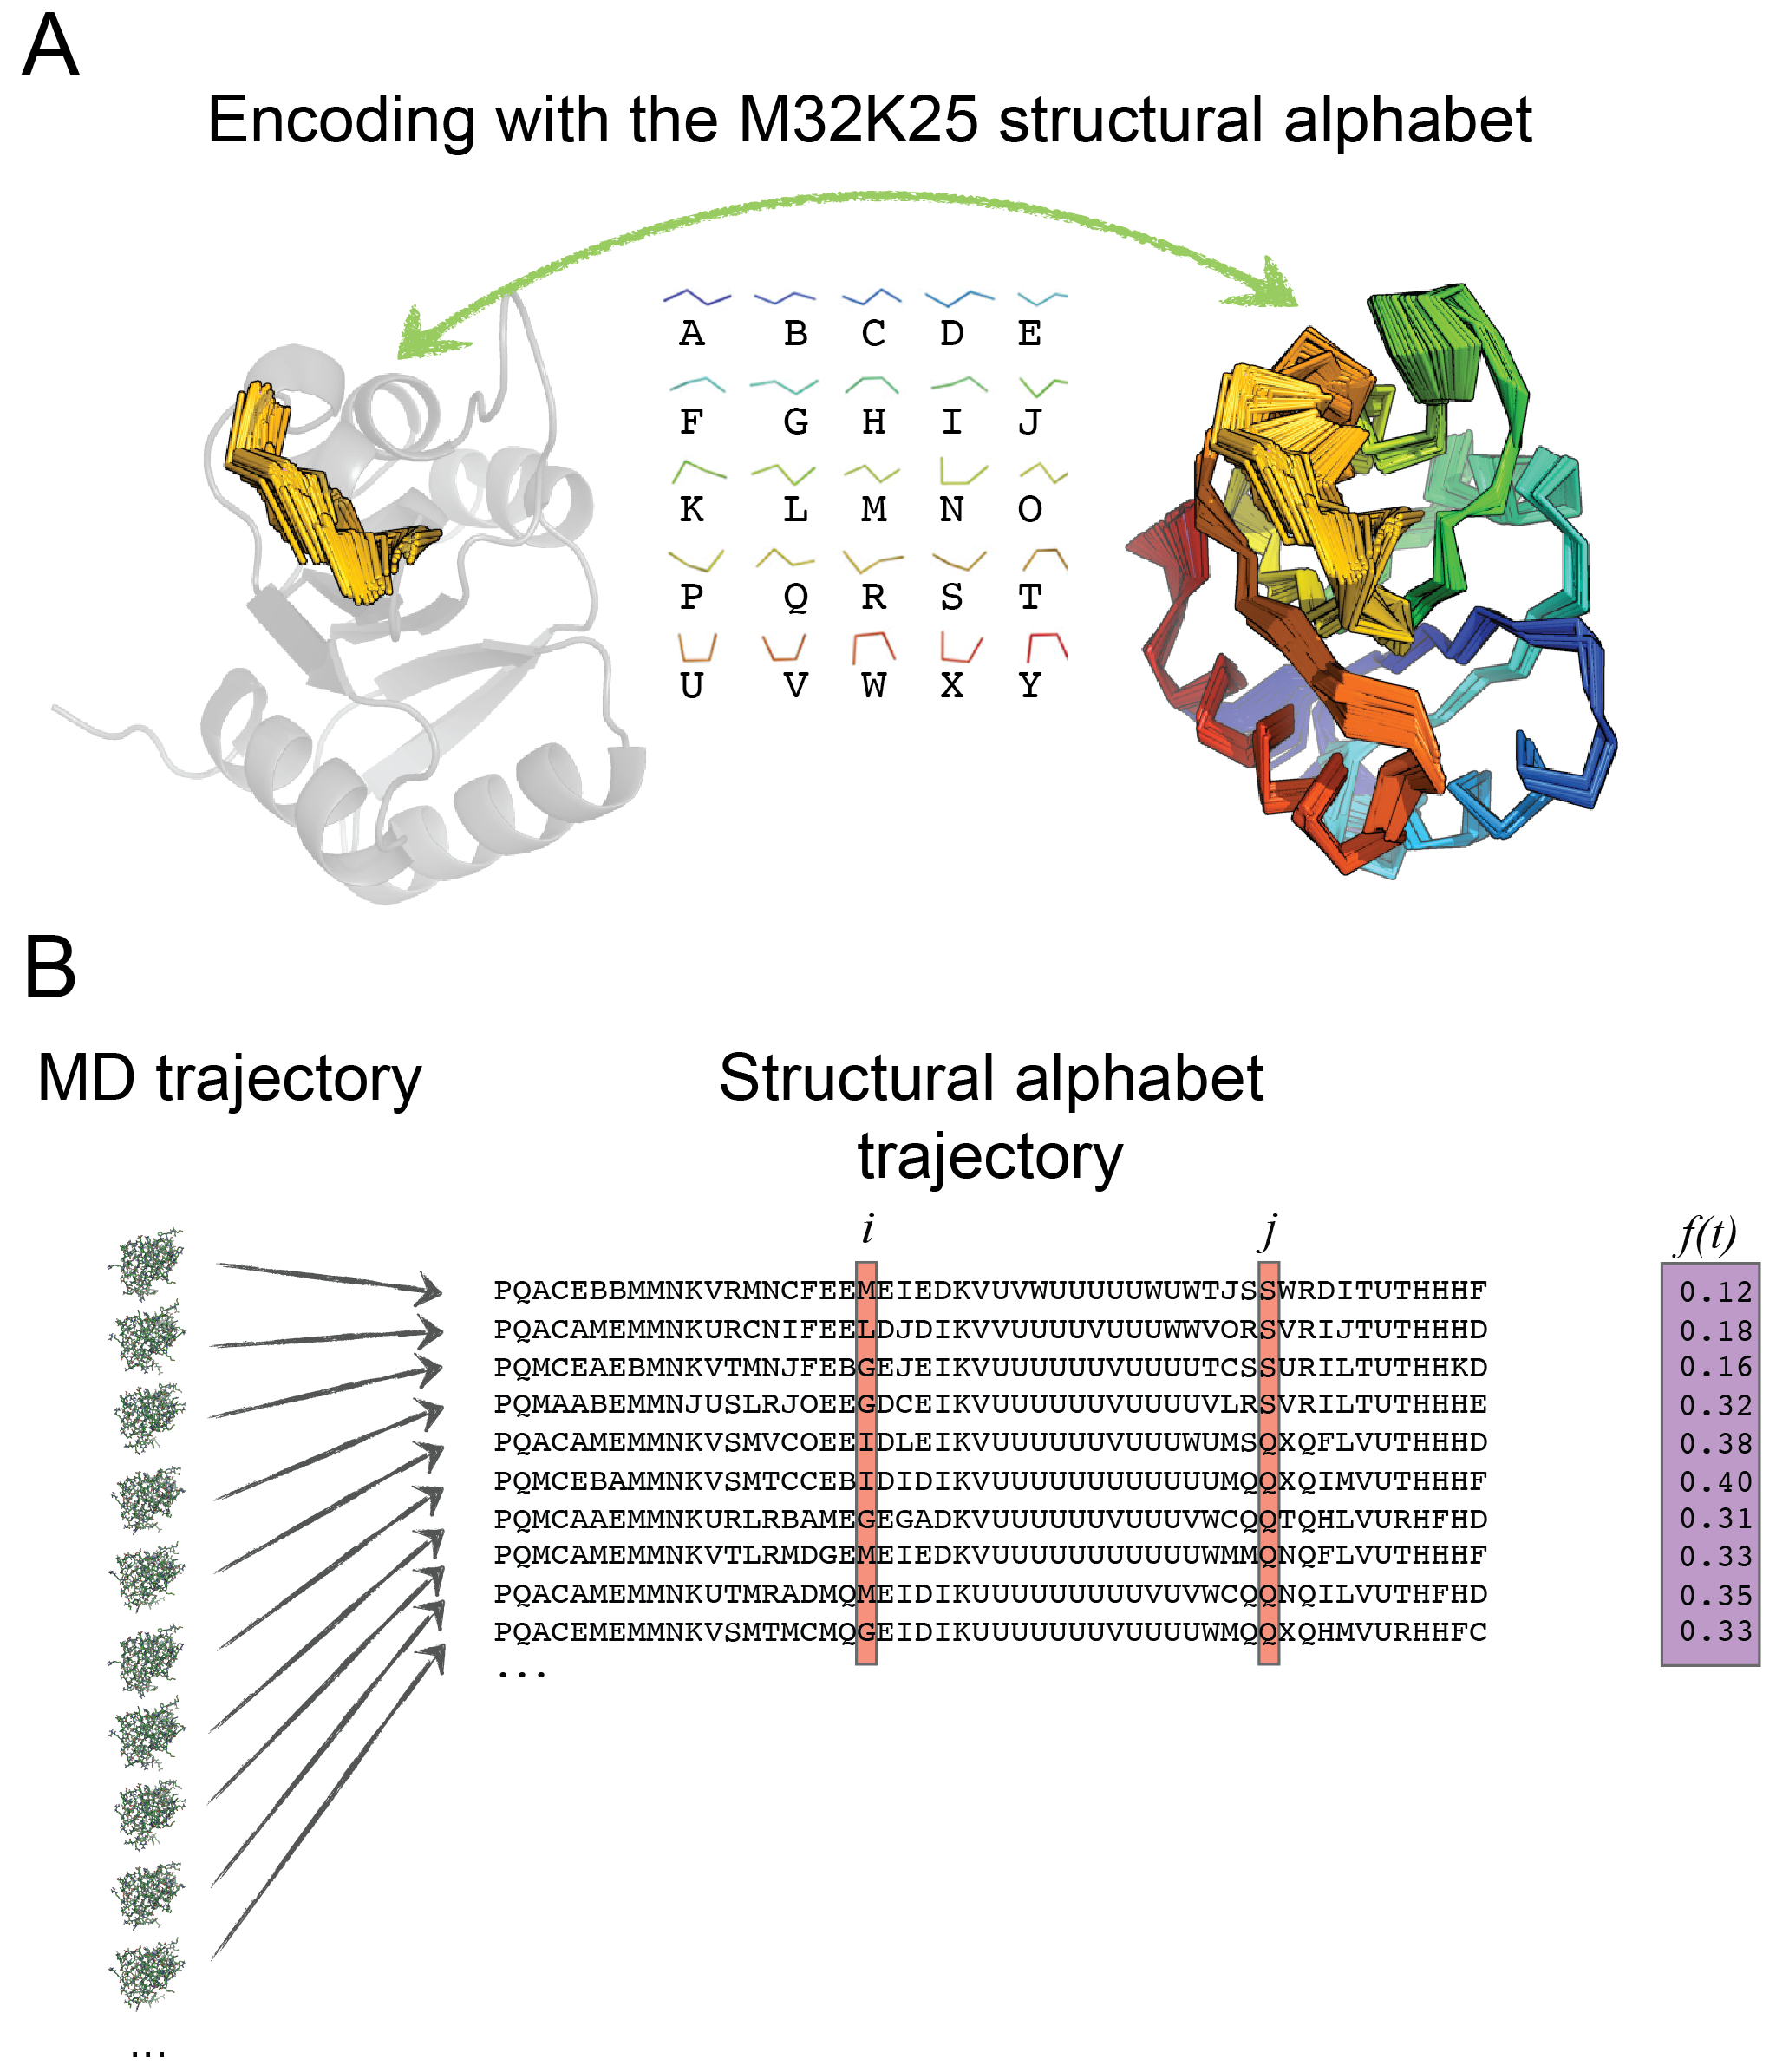
\includegraphics[scale=0.6]{structural_alphabet.png}
\caption[The M32K25 structural alphabet as a fragment-based representation of protein structure and dynamics.]{\textbf{The M32K25 structural alphabet as a fragment-based representation of protein structure and dynamics.} \textbf{(A)} An illustration of the fragment-encoding procedure, whereby a protein is encoded with the M32K25 structural alphabet. Each sequential four-residue stretch is encoded with one of 25 fragments, previously defined by Pandini \textit{et al.} (2010) \cite{Pandini:2010aa}. \textbf{(B)} Multiple conformational snapshots, derived from a molecular dynamics trajectory, are encoded with a string of fragments giving a multiple sequence alignment of the conformational state of each snapshot in the trajectory. The mutual information between each fragment in the protein is then determined by calculating the marginal probabilities and the paired probabilities for each combination of columns in the alignment. This figure is partially reproduced with permission of Dr. Alessandro Pandini.}
\label{fig:sa_encoding_analysis}
\end{figure}
%
%
%
\clearpage
Pandini \textit{et al.} (2012) \cite{Pandini:2012aa} used the M32K25 structural alphabet to encode the ensemble of structures calculated from molecular dynamics simulations of the bacterial two-component system NtrC, as a basis for computing the mutual information between distal fragments in the protein. The authors found that the transmission from the phosphorylation site to the signalling surface of the receiver domain NtrC was mediated by a layer of hub residues \cite{Pandini:2012aa}. Moreover, the location of the hubs preferentially connected to the allosteric site was found to be in close agreement with key residues experimentally identified as involved in the signal transmission.
%
%
\\\\
%
%
A recent investigation of the allosteric mechanism of a myosin small-molecule activator omecamtiv mecarbil (OM) binding to cardiac myosin, used the discrete-state mutual information approach developed by Pandini \textit{et al.} (2012) \cite{Pandini:2012aa} to investigate the mechanism of action of myosin activation. Hashem \textit{et al.} (2017) \cite{Hashem:2017aa} found that OM binding to an allosteric pocket both increased coupling of the motions of the converter and lever arm subdomains to the rest of the protein, and established allosteric communication pathways between the OM binding site and the functional regions in the U50K subdomain. This case-study, and others \cite{Fornili:2013aa,Motta:2018aa,Pandini:2012aa,Pandini:2013aa,Pandini:2015aa,Pandini:2016aa}, demonstrates the utility of discrete-state mutual information as a predictor of allosteric pathways. 
%
%
\\\\
%
%
An important distinction between the method developed by Pandini \textit{et al.} (2012) \cite{Pandini:2012aa} and the linear mutual information method developed by Lange and Grubmueller (2006) \cite{Lange:2006aa}, is that the Pandini \textit{et al.} method normalises the mutual information between fragments by the combined entropies. Determining the positional entropies of fragment-encoded structures is trivial with a discrete-state model (see Equ. \ref{equ:positional_entropy1}), and can therefore easily be computed over each fragment in the structural alignment. Conversely, the method by Lange and Grubmueller calculates the mutual information in Cartesian space. Therefore, it would be necessary to assume the quasi-harmonic approximation in order to compute the positional entropy, offsetting the advantages of mutual information as a statistical framework. Normalising for the combined entropy of each combination of fragments has the presumed effect of reducing false-positives by normalising for random entropic motions, though a robust comparison between the two methods is lacking. Nevertheless, due to the ease of normalising the correlations for random thermal fluctuations within a discrete-state model, the method developed by Pandini \textit{et al.} (2012) \cite{Pandini:2012aa} holds particular promise for revealing allosteric communication pathways. 
%
%
\\\\
%
%
Computer simulations of protein dynamics, including molecular dynamics (MD) stochastic dynamics (SD) and Monte Carlo (MC) simulations, continue to provide a powerful toolbox for the investigation of allosteric transitions. An ensemble view of protein allostery \cite{Motlagh:2014aa} predicates that proteins sample an ensemble of conformations and that the configurational landscape is modified by allosteric ligand binding. This landscape reconfiguration is achieved by pathways of correlated residues, which can be accurately determined by computing the mutual information between distal residues. Nevertheless, each minima in the configurational landscape accessible to a protein gives rise to unique structural and dynamic properties, and therefore measurements of correlated motions should account for this sampling of phase space, though no methods to this end exist. Given the power of trajectory methods for elucidating allosteric transitions, the present work makes use of molecular dynamics simulations to probe the conformational dynamics of PKM2.
%
%
\begin{tcolorbox}
\textbf{Question 3}: To what extent can networks of correlated motions, extracted from defined conformational sub-states, be used as a means of predicting protein residues that propagate the energetic effects of allosteric ligands?
\end{tcolorbox}

\clearpage

\section{Summary of research questions and the contribution of this thesis}
Understanding the molecular basis for how PKM2 catalytic activity is regulated is critical towards investigating its role as a disease target. This thesis follows on from work by Christofk \textit{et al.} (2008) \cite{Christofk:2008ab}, Anastasiou \textit{et al.} (2011) \cite{Anastasiou:2011aa} and Anastasiou \textit{et al.} (2012) \cite{Anastasiou:2012aa} detailing how reduced PKM2 catalytic activity favours pro-tumorigenic cell growth. The prevailing view that allosteric regulation of PKM2 promotes its disease-associated functions was subsequently supported by the a number of compound screens that led to the identification of small molecule activators of PKM2, which were found to alleviate tumour progression by stabilising the highly active tetrameric form of PKM2 \cite{Anastasiou:2012aa}. Additional work by Chaneton \textit{et al.} (2012) \cite{Chaneton:2012aa}, and others, established a cross-talk between glycolysis and \textit{de novo} serine biosynthesis, orchestrated by allosteric regulation of PKM2 by serine and SAICAR. Moreover, work by Morgan \textit{et al.} (2013) \cite{Morgan:2013aa} and more recently by Yuan \textit{et al.} (2018) \cite{Yuan:2018aa} found that PKM2 acts as a nutrient sensor for a number of amino acids, which can activate or inhibit enzyme activity by binding to a common allosteric pocket. Taken together, these studies led us to hypothesise that the cellular activity of PKM2 is regulated by numerous allosteric ligands, and that this may be relevant for metabolic phenotypes associated with cancer cell growth. Allosteric regulation of PKM2 activity by numerous endogenous ligands may occur either in isolation; or concurrently, resulting from the multiplicity of distinct allosteric pockets on the surface of PKM2. While the mechanisms of how PKM2 responds to ligands \textit{per se} has been carefully investigated, very little is understood about how PKM2 responds to simultaneous binding of multiple allosteric effectors with opposing functional signals. This led to the first research question: \textit{Do cellular metabolic conditions exist under which PKM2 is likely to be bound to multiple allosteric effectors? And if so, how are the effects of concurrently bound ligands, with opposing functional signals, integrated by PKM2 to regulate enzyme catalysis?} To this end, Chapter 3 investigates possible functional mechanisms of allosteric regulation by a number of ligands, both alone and in combination, on PKM2 enzyme activity. 
%
%
\\\\
%
%
Regulation of PKM2 enzyme activity has been suggested to involve oligomeric changes and possible subtle conformational rearrangements. Early investigations of PKM2 regulation by Hofmann \textit{et al.} (1975) \cite{Hofmann:1975aa} suggested that the oligomeric structure of the protein can alternate between lower-order oligomers and tetramers. Subsequent work by Kato \textit{et al.} (1989) \cite{Kato:1989aa}, Anastasiou \textit{et al.} (2012) \cite{Anastasiou:2012aa}, Morgan \textit{et al.} (2013) \cite{Morgan:2013aa} and Yan \textit{et al.} (2016) \cite{Yan:2016aa} found that stabilisation of PKM2 tetramers resulted in high enzyme activity. Nevertheless, the monomer-dimer-tetramer distribution of PKM2 in the absence of any allosteric ligands, and the subsequent effects of various ligands on this distribution, is disputed. Moreover, if multiple ligands concurrently regulate PKM2, under cellular metabolic conditions, the necessary relationship between enzyme activity and oligomerisation remains to be determined. It may, for example, be the case that a molecule of PKM2 is bound to both FBP (an activator; reportedly promotes tetramerisation) and alanine (an inhibitor; reportedly destabilises tetramers). Given the current available knowledge in the literature, it is unclear how ligands alone, and in combination, determine the oligomeric state of PKM2, and whether this is linked to the prevailing level of enzyme activity. This led to the second research question, which will be addressed herein: \textit{What are the contributions of ligand-induced conformational and oligomeric changes to PKM2, and what are the relationships between these allosteric effects and PKM2 activity?} The relationship between PKM2 activity and its oligomeric state is of greater biological interest given that PKM2 activity in cells is often inferred from the its oligomeric state \cite{Anastasiou:2011aa,Anastasiou:2012aa,Christofk:2008ab,Hitosugi:2009aa,Lim:2016aa,Wang:2017aa,Wang:2017ab}. To this end, Chapter 4 presents an investigation of the oligomeric and structural conformation of PKM2, and how this changes in response to concurrent allosteric ligand binding, using native mass spectrometry and ion mobility. Chapter 5 builds on the experimental findings of the previous chapter, and presents details about the conformational dynamics of PKM2 in response to allosteric regulation, gleaned from molecular dynamics simulations.
%
%
\\\\
%
%
The previous finding by Anastasiou \textit{et al.} (2012) \cite{Anastasiou:2012aa} that allosteric activation of PKM2 alleviates some of its pro-tumourigenic functions, suggests that genome-encoded, and therefore stably propagated, allosteric effects can contribute towards disease progression. Allosteric pockets are subject to less evolutionary pressure and hence are more sequence variable than orthosteric sites \cite{Yang:2012aa}, affording exogenous allosteric ligands greater target specificity. Therefore, methods which [i] identify putative allosteric pockets and [ii] elucidate networks of protein residues involved in the propagation of allosteric signals, would hold great power for drug discovery. Particularly successful has been the use of analysis methods such as those developed by Pandini \textit{et al.} (2012) \cite{Pandini:2012aa} and Lange and Grubmueller (2006) \cite{Lange:2006aa} used to identify distally correlated 	motions in the backbone of proteins in order to elucidate allosteric pathways. Nevertheless, work by Volkman \textit{et al.} (2001) \cite{Volkman:2001aa}, Lindorff-Larsen \textit{et al.} (2005) \cite{Lindorff-Larsen:2005aa}, Yao \textit{et al.} (2008) \cite{Yao:2008aa}, Guerry \textit{et al.} (2013) \cite{Guerry:2013aa} and many others, has shown that protein dynamics results in an ensemble of pre-existing conformations that determine the physico-chemical and functional properties of enzymes. In this respect, ensemble-averaging of any dynamic time-resolved observable is required. Additional methods are required to predict the network of residues involved in protein allostery, with a consideration for the ensemble nature of protein dynamics. This led to the third and final research question: \textit{To what extent can networks of correlated motions, extracted from defined conformational sub-states, be used as a means of predicting protein residues that propagate the energetic effects of allosteric ligands?} To address this question, Chapter 5 presents the development of a \textit{AlloHubMat}, a novel method and stand-alone software package used to predict allosteric hub residues from molecular dynamics simulations using tools from information theory. AlloHubMat is applied towards the analysis of molecular dynamics simulations of PKM2 and predicts a network of residues involved in propagating the effects of FBP-induced activation. These \textit{in silico} predictions are tested in Chapter 6 using single-point mutant variants of PKM2, designed to abrogate the allosteric pathways induced by FBP activation.
%
%
\\\\
%
%
In addition to various biophysical and analytical methods, molecular dynamics simulations are used as a detailed statistical-mechanical technique for investigating the conformational dynamics of PKM2 in response to allosteric regulation. Moreover, the simulated trajectories generated from MD calculations are used as an input for AlloHubMat, to predict allosteric pathways. Given the importance of molecular dynamics as an \textit{in silico} tool for this work, and the immense power it presents for the study of protein dynamics, the mathematical and physical principles of MD simulations are detailed in the following Chapter. 
%
%
%%% FIGURE
%
\begin{figure}[!ht]
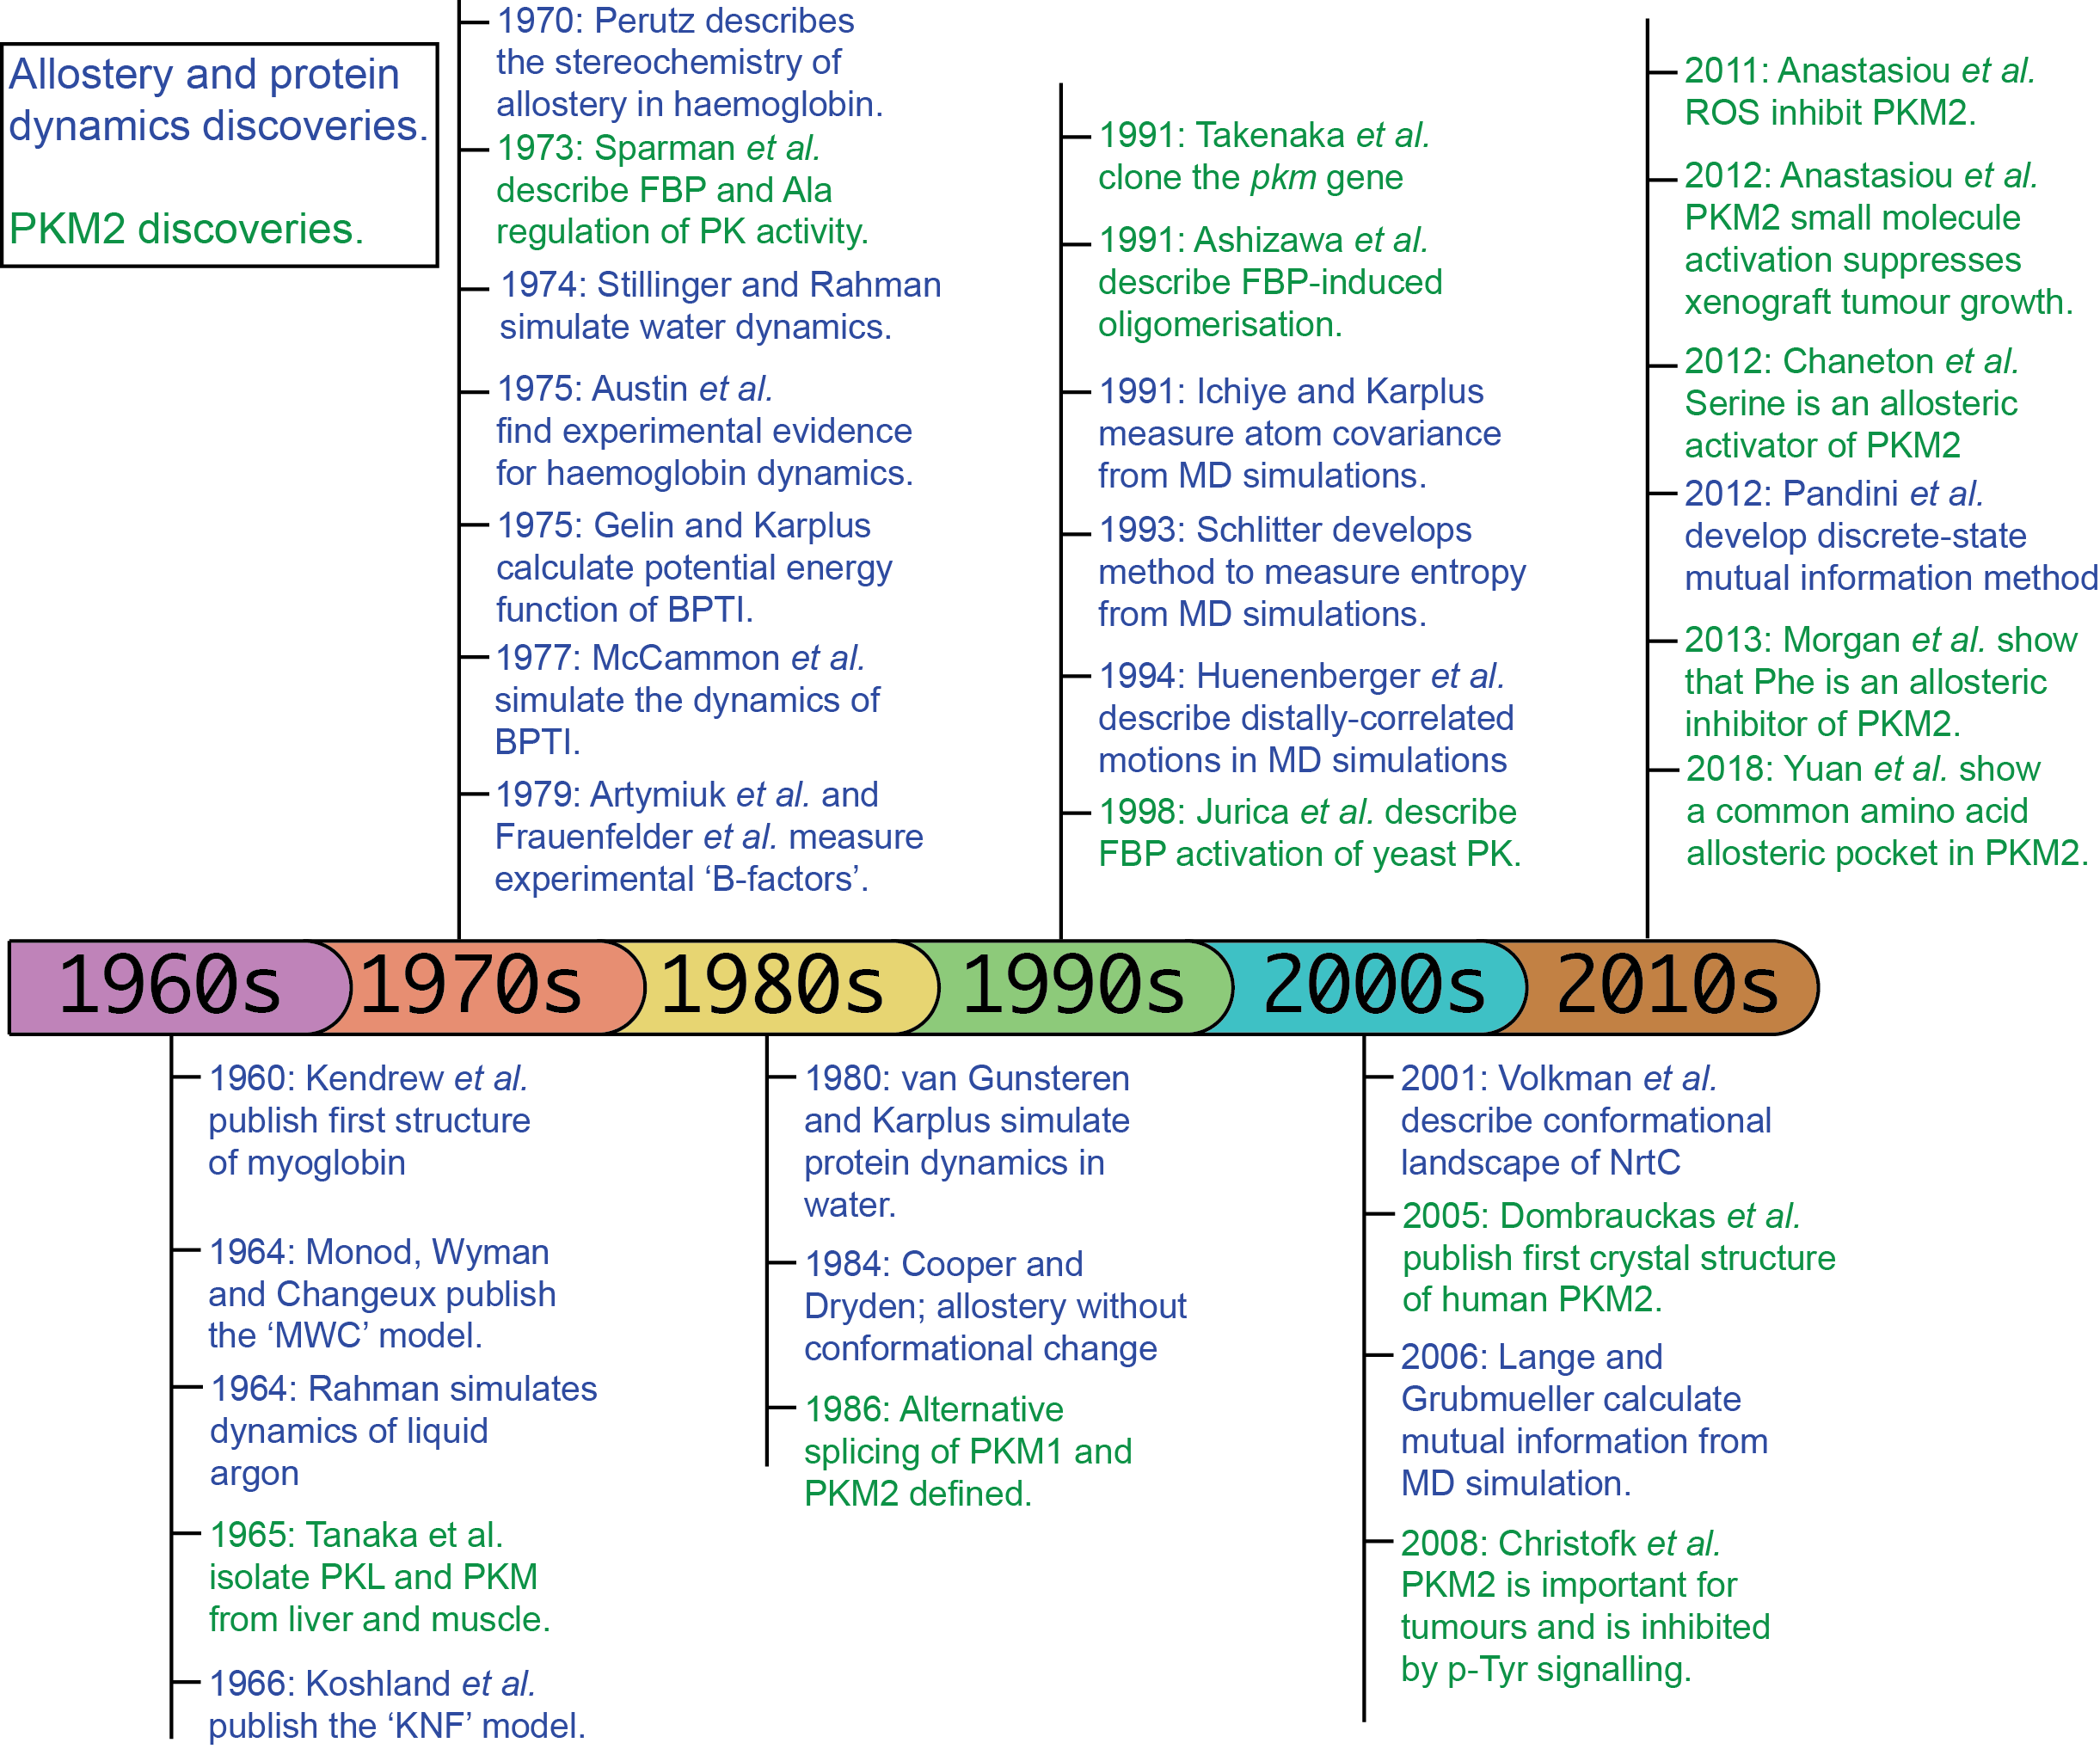
\includegraphics[scale=0.7]{historical_timeline.png}
\caption[Time line of historical discoveries in the fields of protein dynamics and allostery, and PKM2 biology and biophysics.]{\textbf{Time line of historical discoveries in the fields of protein dynamics and allostery, and PKM2 biology and biophysics.} Historical discoveries relating to the fundamental concepts of protein dynamics and allostery, with a focus on molecular dynamics simulation methods, are shown in dark blue. Discoveries relating to PKM2 biology, structure and regulation are shown in dark green. }
\label{fig:timeline}
\end{figure}
%
%
\clearpage





















  

